%\setcounter{chapter}{7}
\chapter{Module Production for the Phase I CMS Pixel Detector Upgrade}\label{ch:phase1}

As discussed in chapter \ref{ch:lhcandcms} the CMS pixel detector will \ital{suffer} from radiation damage throughout its lifetime hence the need for periodical updates. The first version of the detector was known as phase 0, it became fully operational 2010 after solving a setback during the original starting period in 2008. In 2017 the pixel detector was replaced during the so-called phase 1 upgrade, the University of Nebraska, high energy group (UNL-HEP) played a major role in assembling and testing over 500 modules, from 2013 to 2016, which then became part of the forward region of the pixel detector (FPix). The next update of this detector (phase 2) is projected to take place in 2025 when the current detector will be reaching its limits. In this chapter we describe why the phase 0 pixel detector needed an upgrade making 

the work done by the UNL-HEP group. Some of these steps will be highlighted and described in detail as they were my contributions to this production campaign. Specially the  and highlighting 

\section{The CMS Pixel Detector Phase I Upgrade}
The CMS pixel detector is composed of two sections, the barrel section (BPix) and the forward section (FPix). Each of these sections (for phase 0) was composed of three layers originally designed to record three 3D positions (tracks) of the particles emerging from the \ital{pp} collisions. As well as to provide information to reconstruct primary and secondary vertices of decaying particles. This detector performed well during the LHC run I,{\rojo{incorporate the bunch crossing?}} taking data at the design luminosity of $1 x 10^{34} cm^{-2} s^{-1}$, which was then used in many analysis including the discovery of the Higgs bosson published in 2013. But after a few years of operation the pixel detector started to degrade due to radiation damage, causing an increase of fake rates as well as loose on resolution. Moreover, for run II the LHC planned to double the luminosity with successive increment until reach its peak of $2 x 10^{35} cm^{-2} s^{-1}$. A simulation of the performance of the pixel detector under different luminosity conditions can be seen in figure \ref{fig:red_perf}

\begin{figure}[!h]
\centering
\includegraphics[width=0.9\textwidth]{ch7/reducedperformance}
%\includegraphics[width=0.9\textwidth]{pixel/reducedperformance}
\caption[Expected performance of the original pixel detector for different luminosities.]{Expected performance of the original pixel detector under different luminosity conditions: a) track-finding efficiency; b) fake rate. Conventions are the same for both plots, considering zero pileup (blue squares), average pileup of 25 (red dots), average pileup of 50 (black diamonds), and average pileup of 100 (magenta triangles).\cite{pix_tdr}}\label{fig:red_perf}
\end{figure}

This degradation prompted the need for an improved pixel detector. It was designed to have four layers in the barrel ubicated at distances of Hena2420
and 3 layers at each endcap as shown in \ref{fig:new_pix}. better 

{\rojo{This degradation prompted the need for an improved pixel detector. It was designed to have four layers in the barrel ubicated at distances of Hena2420
and 3 layers at each endcap as shown in \ref{fig:new_pix}. better }}

{\rojo{This degradation prompted the need for an improved pixel detector. It was designed to have four layers in the barrel ubicated at distances of Hena2420
and 3 layers at each endcap as shown in \ref{fig:new_pix}. better lllllllllllll l l l l lll ll l l l ll l l l ll l lllllllllllllllllllllllllllllll lll l ll l l ll ll ll lll llll llll lll llll lll lll lll lllll lll llllll lllll lll llll llll llll lllll lll ll l l l ll pasa hacer espacio tenemos que escribir vainas mas coherentes a ver si ahora si slata la pagina}}

\begin{figure}[!h]
\centering
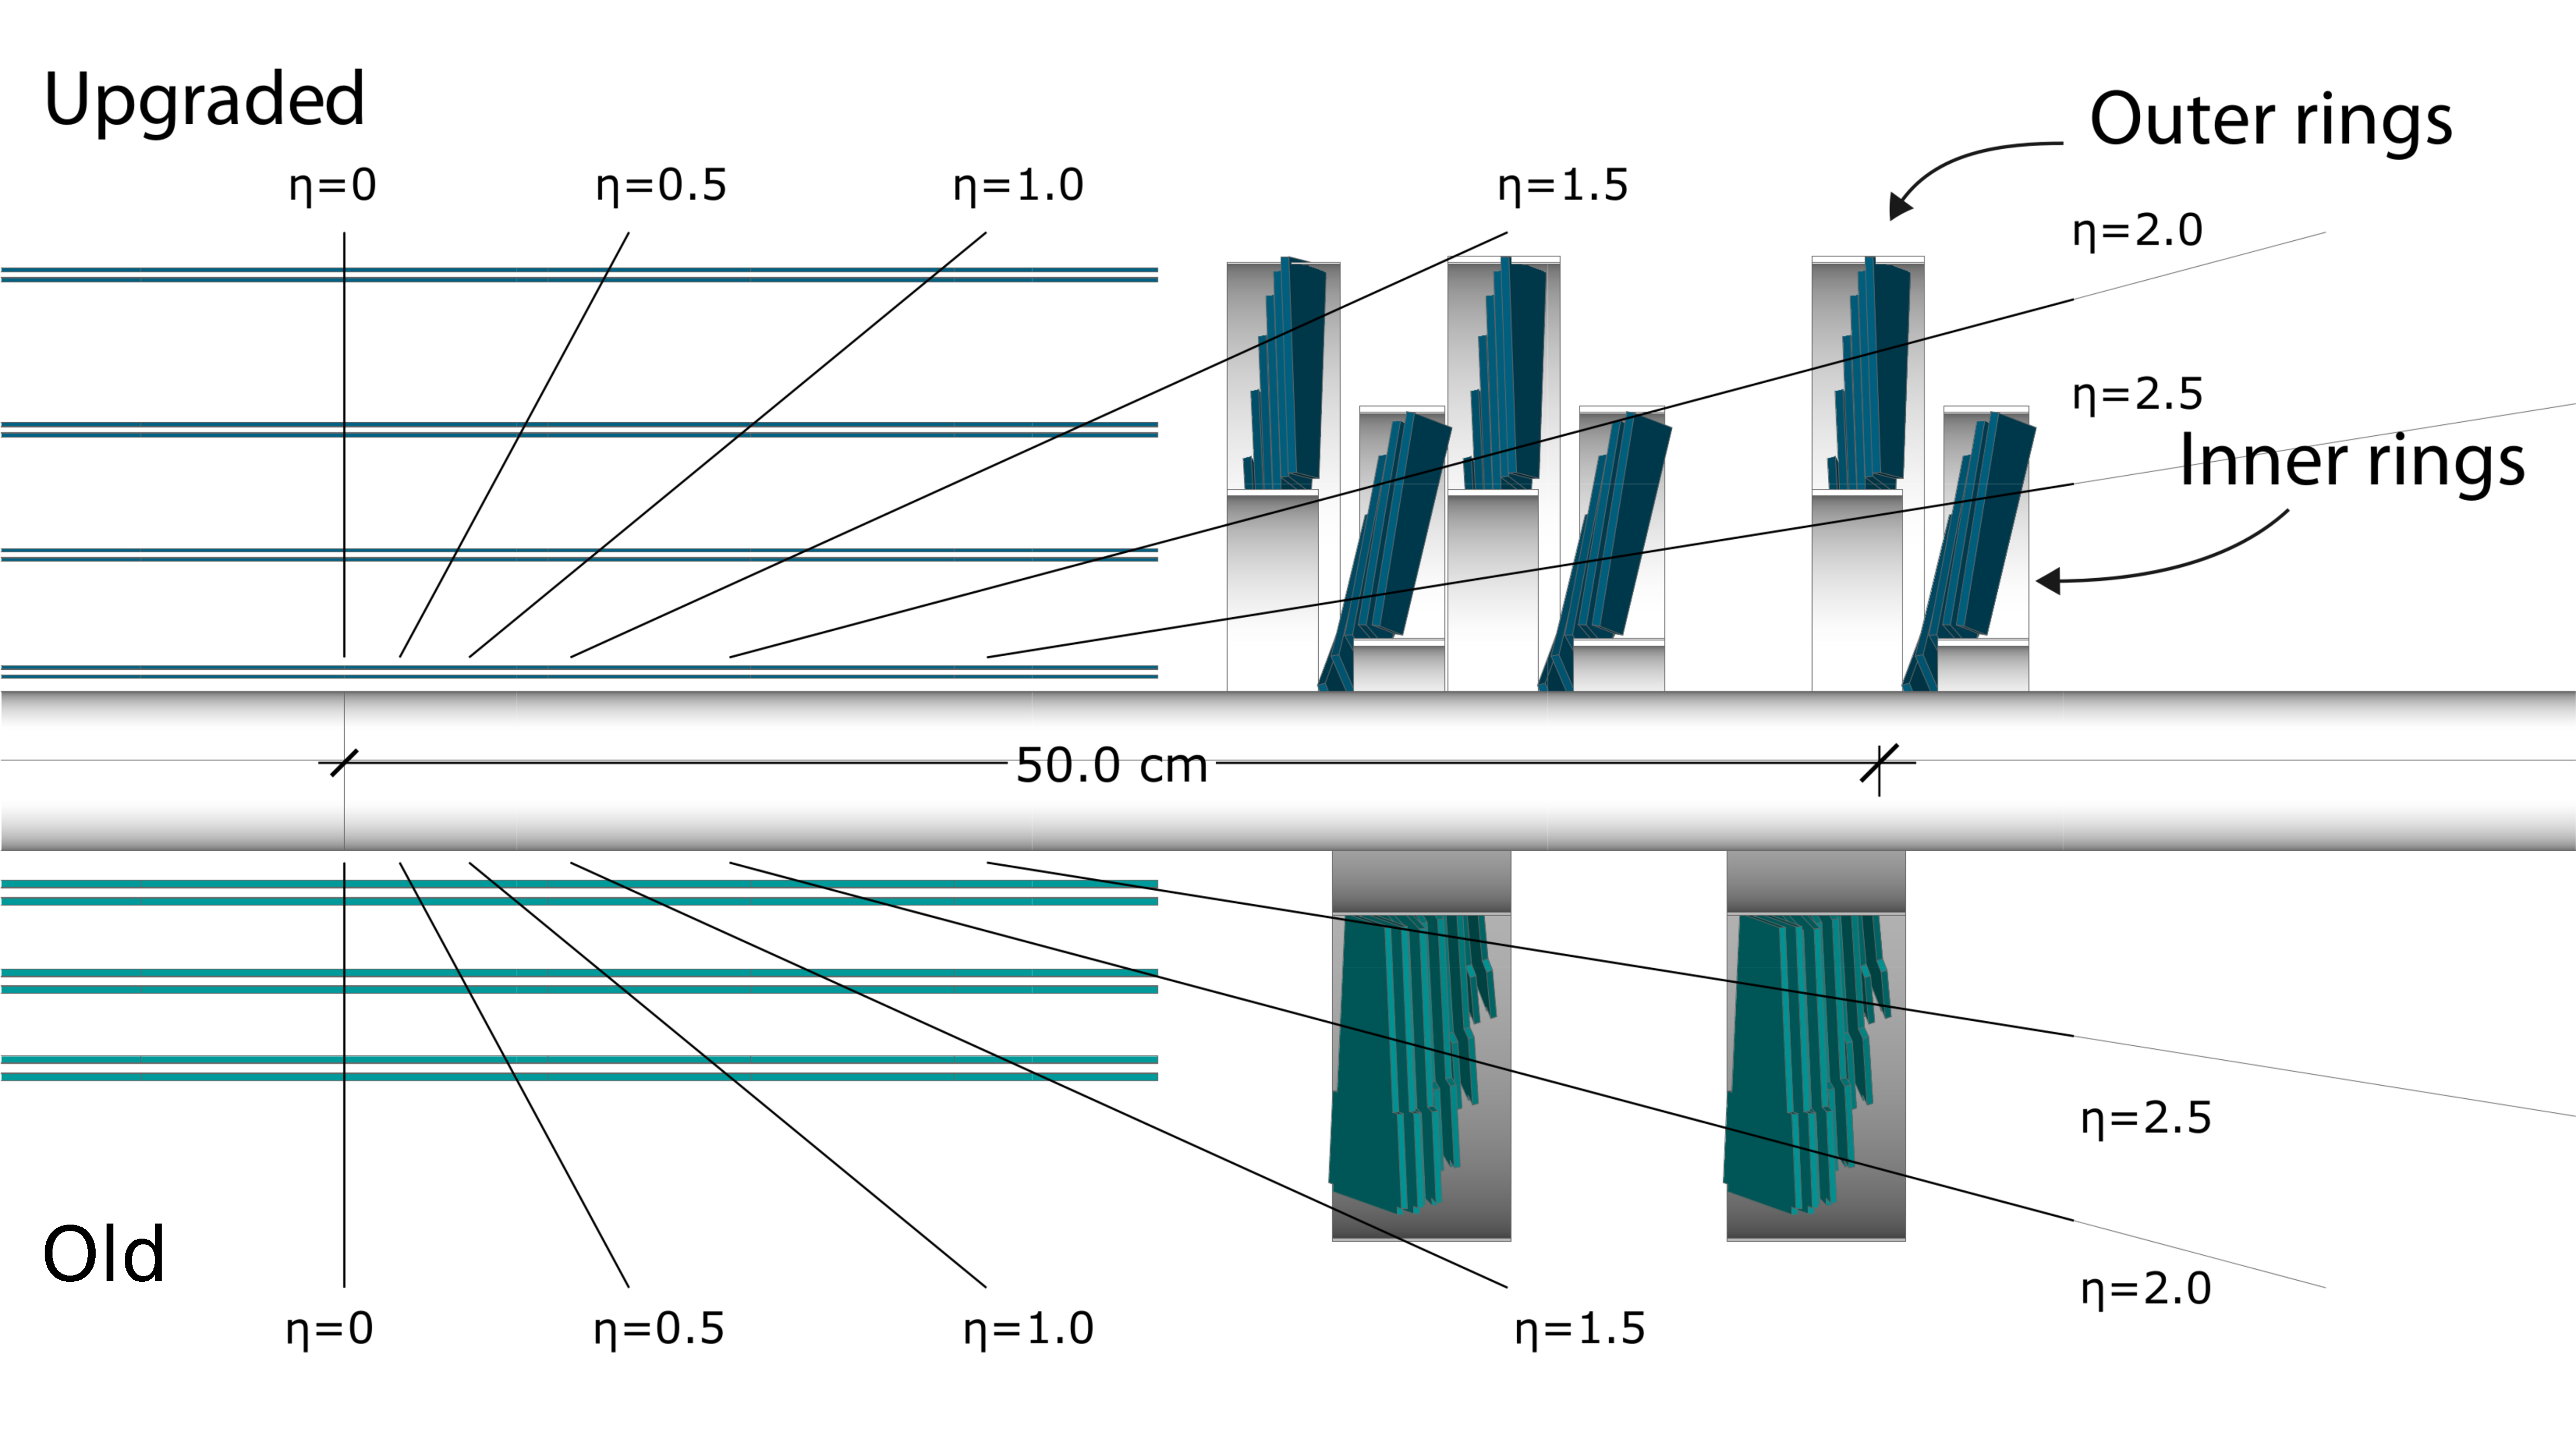
\includegraphics[width=0.6\textwidth]{../images/ch7/fpix.pdf}
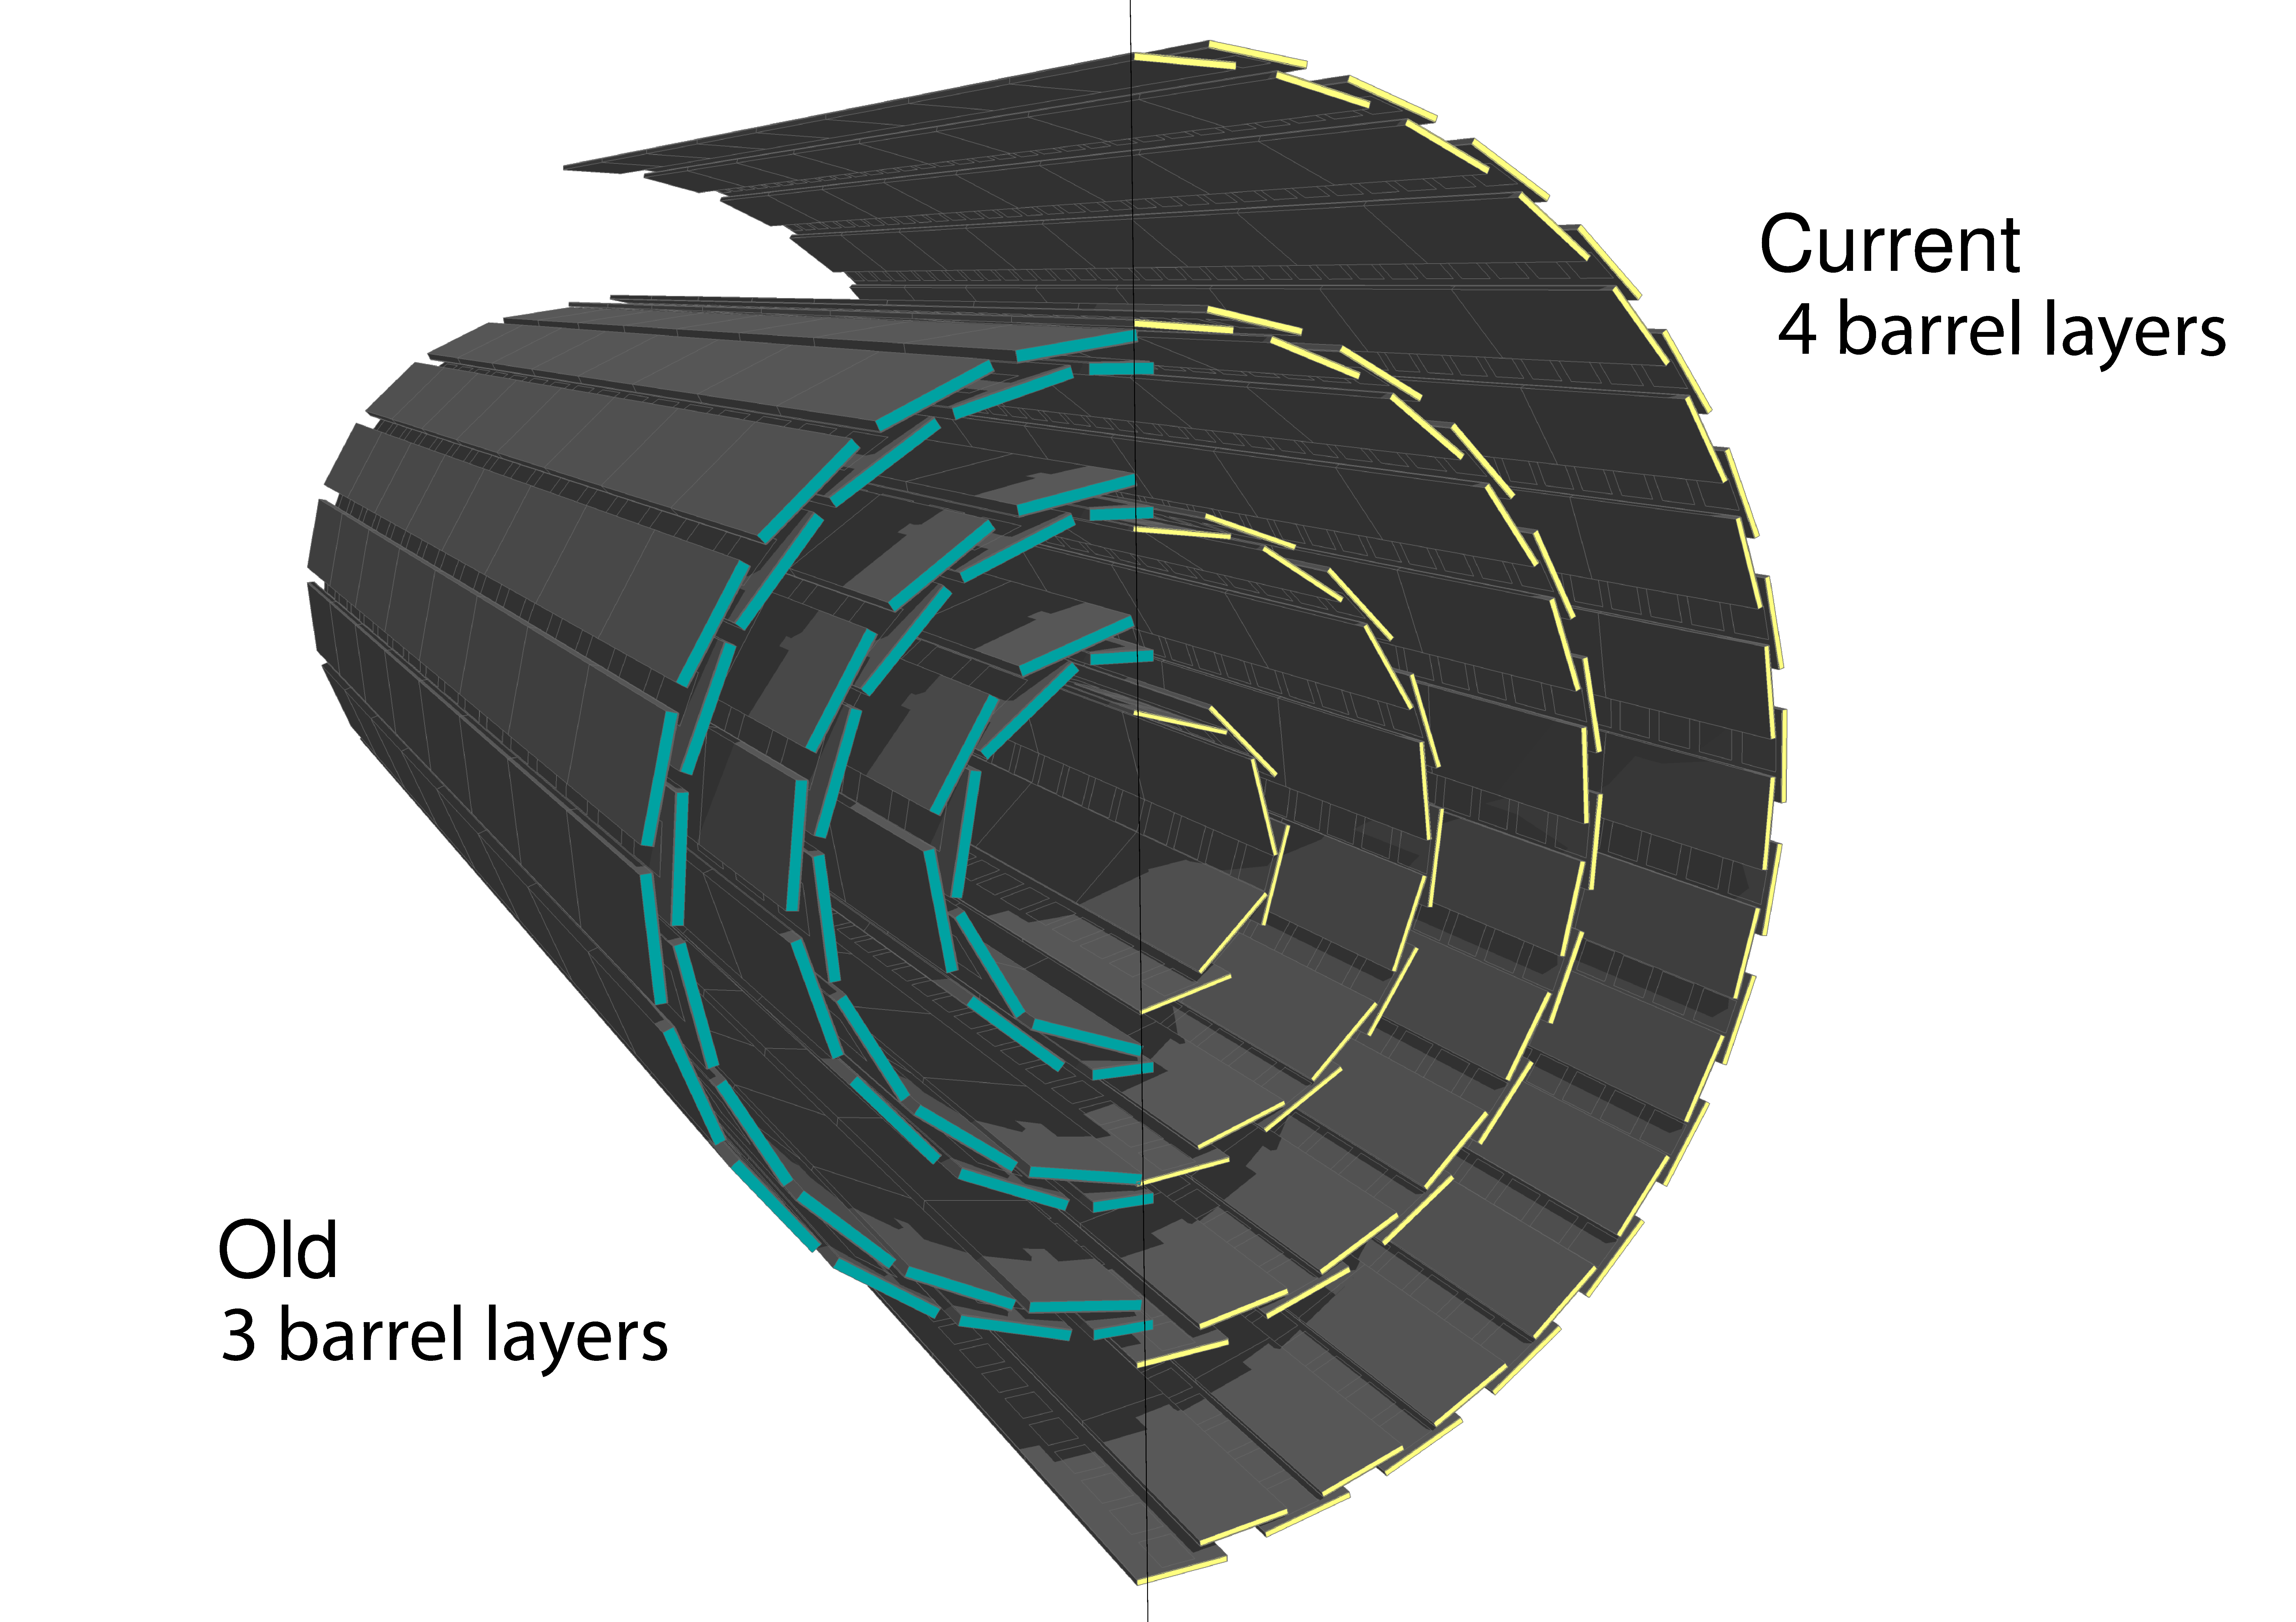
\includegraphics[width=0.39\textwidth]{../images/ch7/bpix.pdf}
\caption[Layout of the upgraded and old pixel detectors.]{Layout and comparison of the layers and disks in the upgraded (Phase I) and old (Phase 0) pixel detectors \cite{pix_tdr}.}\label{fig:new_pix}
\end{figure}

%%%%%%%%%%%%%
%%%%%%%%%%%%
%%%%%%%%%%

\section{Module Production at UNL}
The UNL module production workflow was designed to follow a pipeline-like structure as shown in figure \ref{fig:unlworkflow}. 

\begin{figure}[!h]
  \centering
  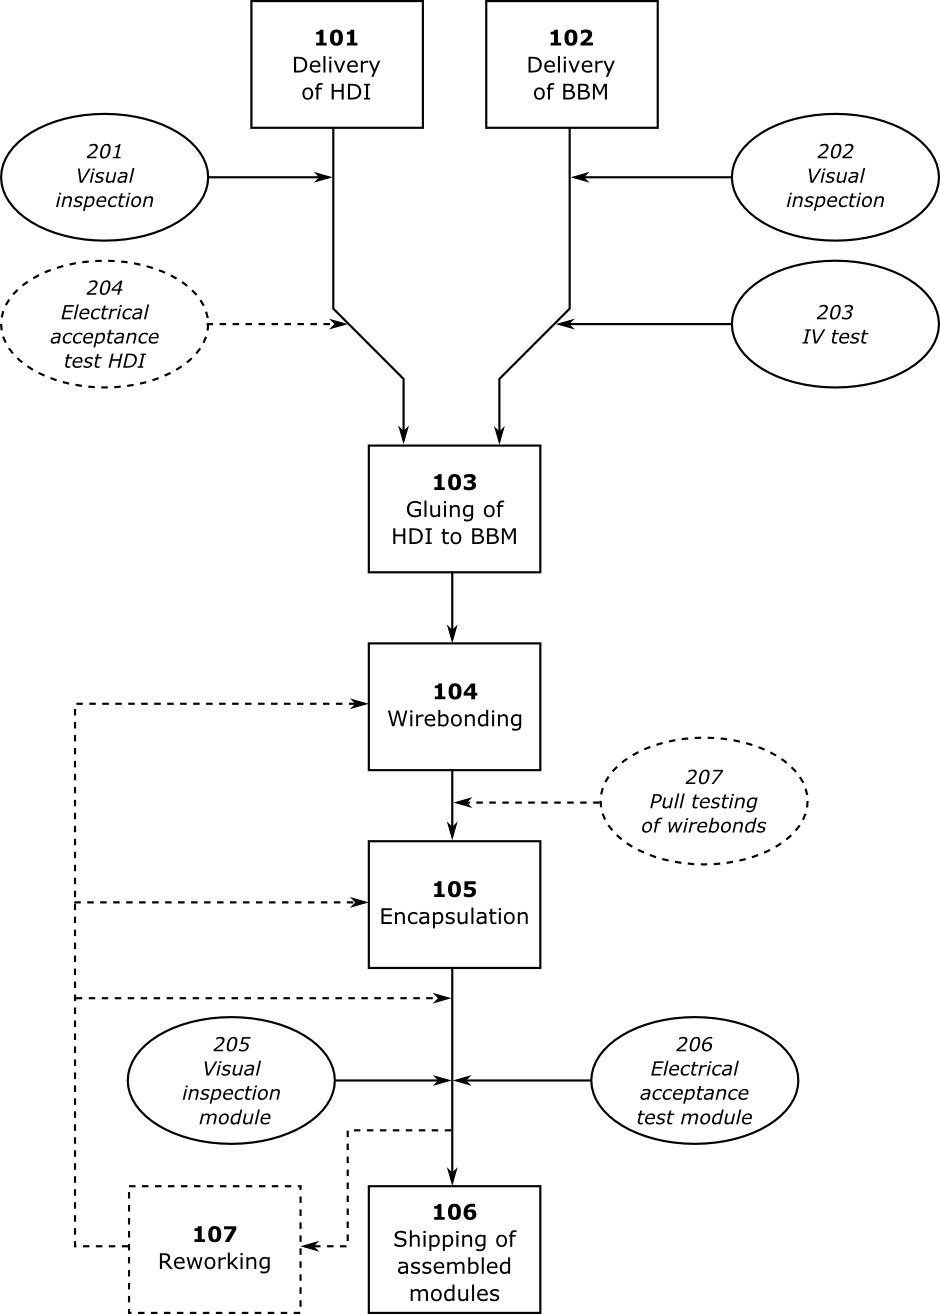
\includegraphics[width=0.7\textwidth]{../images/ch7/unl_workflow}
  \caption[UNL module assembly workflow.]{UNL module assembly workflow. Dashed lines represent occasional quality testing and reworking procedures\cite{ph1_sop}.}\label{fig:unlworkflow}
\end{figure}

This allows for different batches of modules to be going through it at different stages without stopping the workflow. Following is a short description of the tests and procedures performed during the production in the UNL silicon Lab. Special emphasis will be made in IV test, visual inspection and electrical test, the stages where the author of this work made most of the work{\rojo{improve}}. 

\subsection{Visual Inspections}
The UNL-HEP group assembly workflow started upon receiving two components: a Bare Bonded Module (BBM) and a High Density Interconnect (HDI), see figure \ref{fig:bbmyhdi}.

\begin{figure}[!h]
\centering
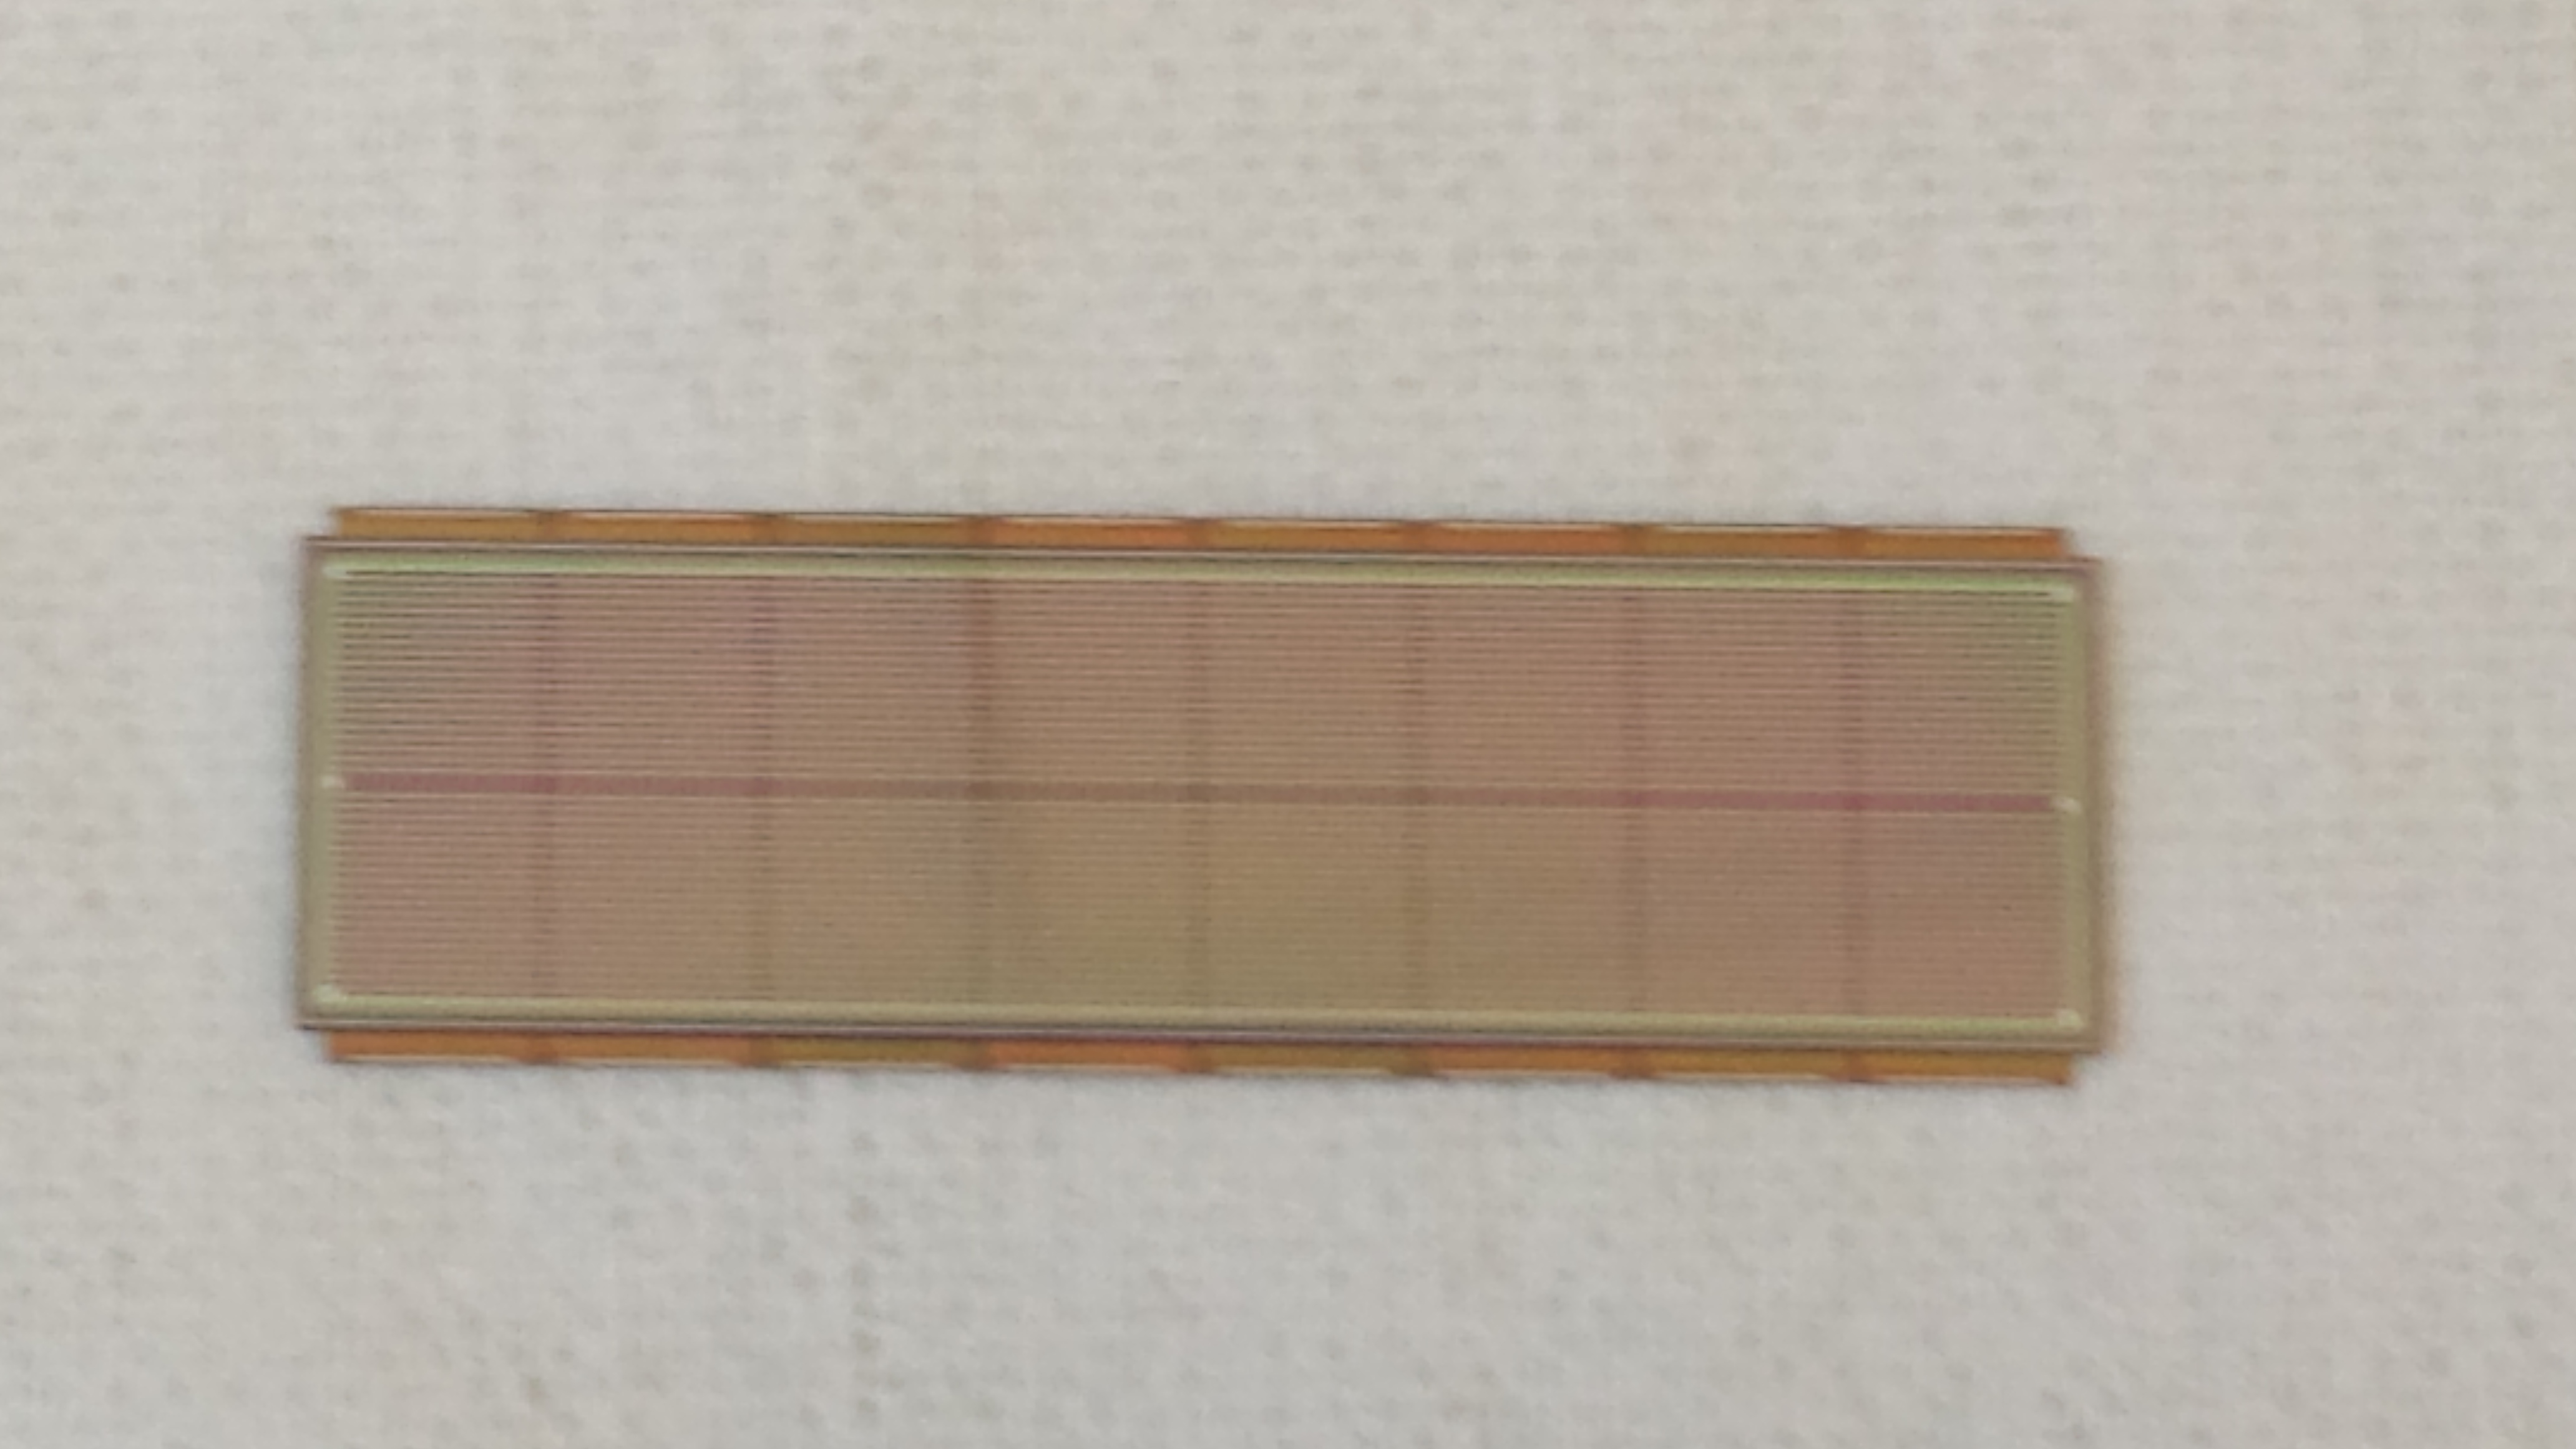
\includegraphics[width=0.6\textwidth]{ch7/bare_module}
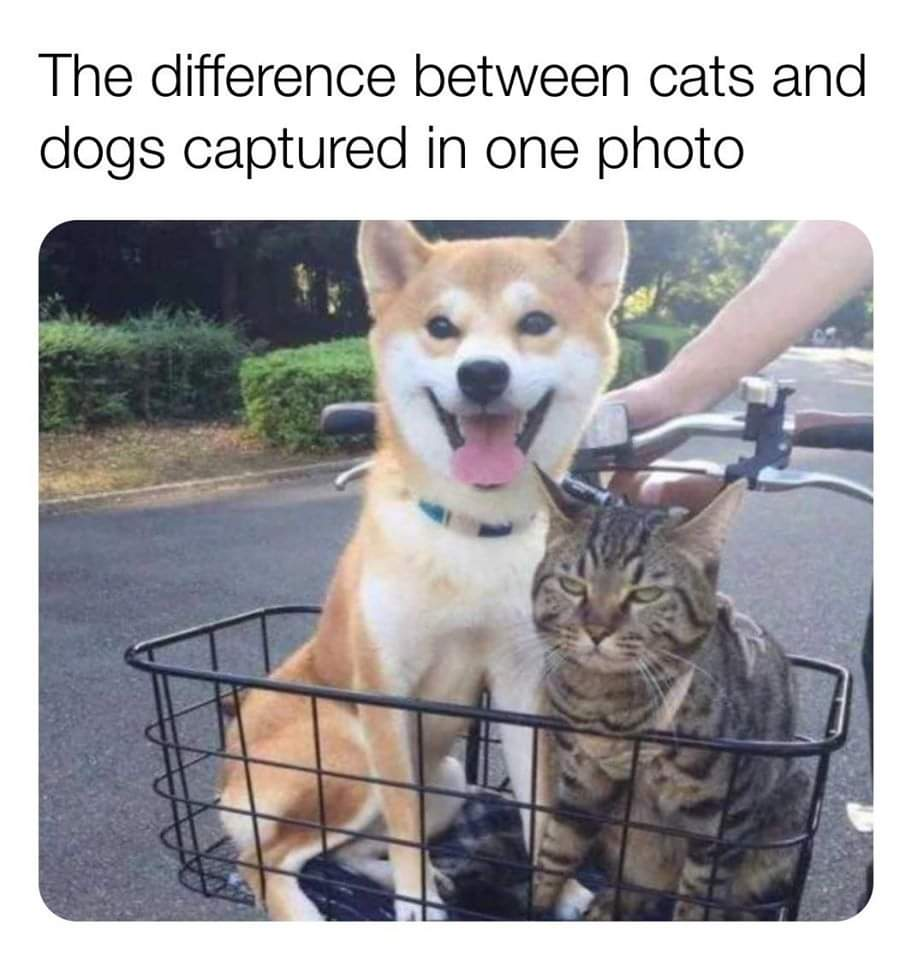
\includegraphics[width=0.39\textwidth]{ch7/gato2}
\caption[Photograph of a BBM and HDI.]{Photograph of a BBM (left) and HDI (right) as received by the UNL-HEP group.}\label{fig:bbmyhdi}
\end{figure}

The first stage of the module production was to do a visual inspection on these components to ensure they were in good conditions and able to continue into the production pipeline. {\rojo{punto aparte?}} To get a good view of such a small components a powerful microscope with magnification of {\rojo{confirm}}, an attached camera, and LED ring illumination was used. A photograph of the set up is shown in figure \ref{fig:iv_station}. BBM were received in a gel pack while the the HDI were usually received in their modules carriers. BBM and HDI were moved from the container into the probe station using a vacuum pen and taking the appropriate safety precaution: ESD wristband, gloves, face mask, etc.

\begin{figure}[!h]
\centering
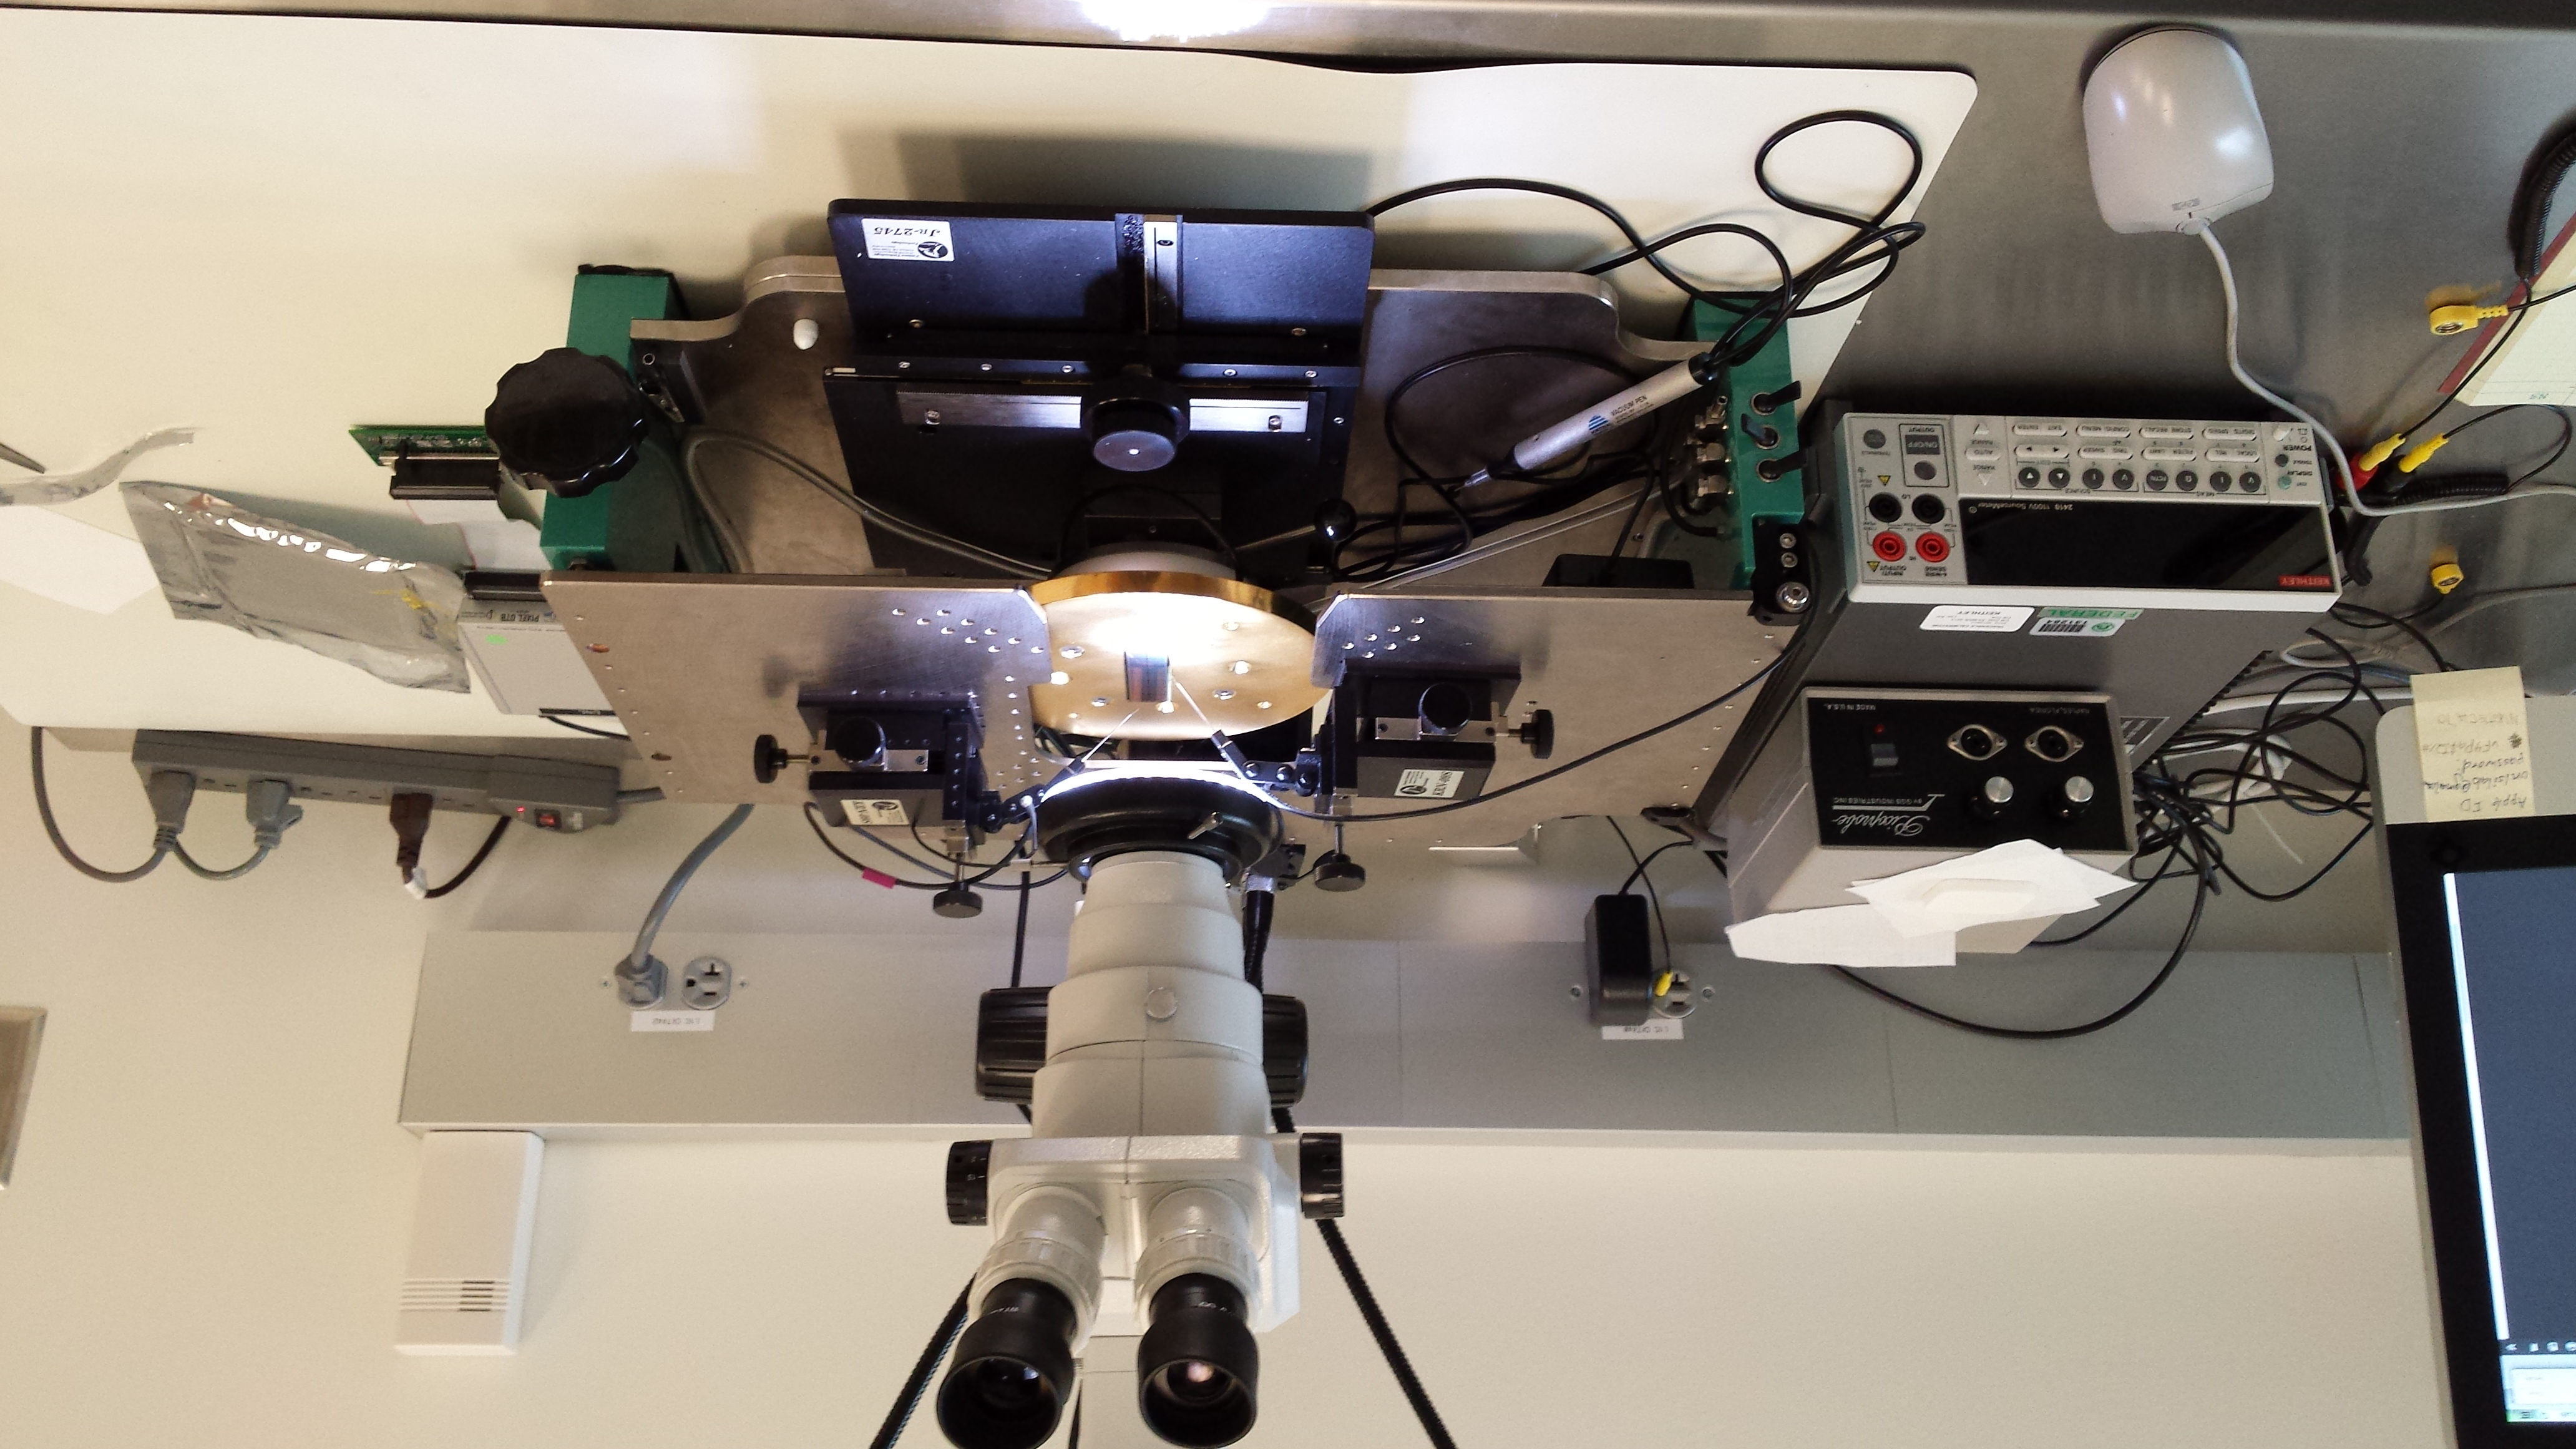
\includegraphics[width=0.7\textwidth]{ch7/iv_station}
\caption[Photograph of the visual inspection and IV test station.]{{rojo{fix}} Photograph showing a BBM under the microscope during a visual inspection. This station also served as IV test stand.}\label{fig:iv_station}
\end{figure}

During visual inspection BBMs were scanned for unusual features or sign of damage, special attention was given to the high voltage connection and bond pads. Figure \ref{fig:vis_insp_bbm} shows different parts of four different modules where defects are observed {\rojo{defects are on only 3}}. Some of these defects, bottom right figure, caused, the module to be rejected immediately while others, top right and bottom left plots, will still undergo an IV test. While for the HDI the bond pads of the 16 ROCs, the wirebonds of the tbm, and the address pads were carefully checked. Figure \ref{fig:vis_insp_hdi} shows the TBM wirebonds as well as the bondpads of a ROC in a HDI.

\begin{figure}[!h]
  \centering
  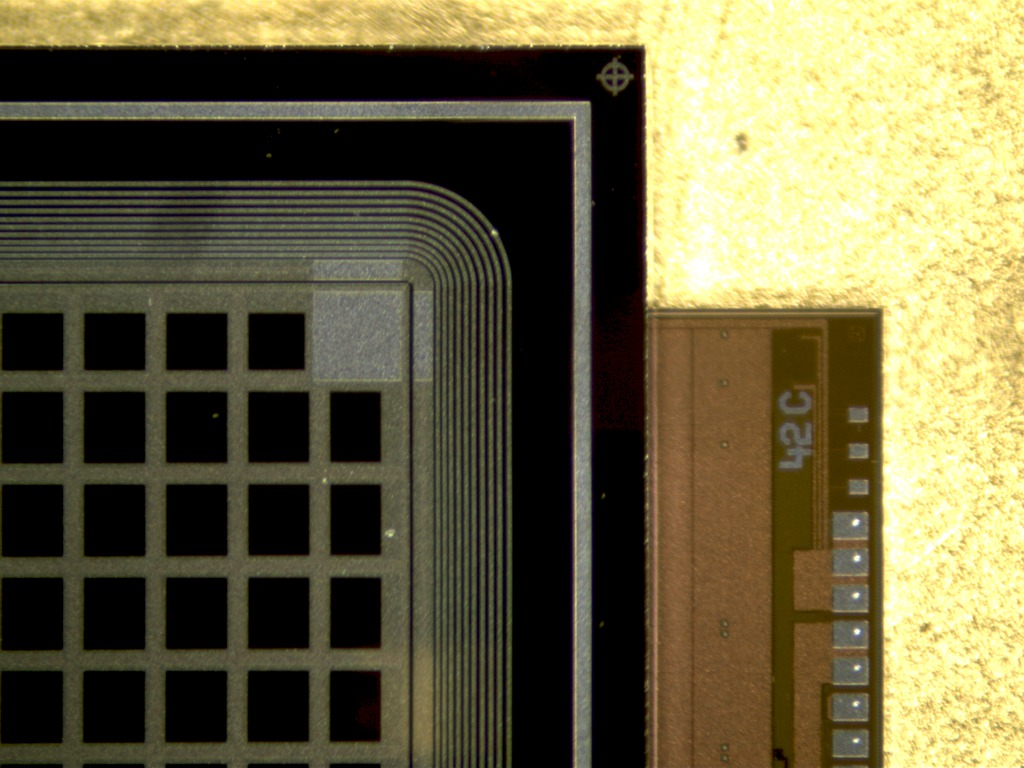
\includegraphics[width=0.4\textwidth]{ch7/vis_insp_1}
  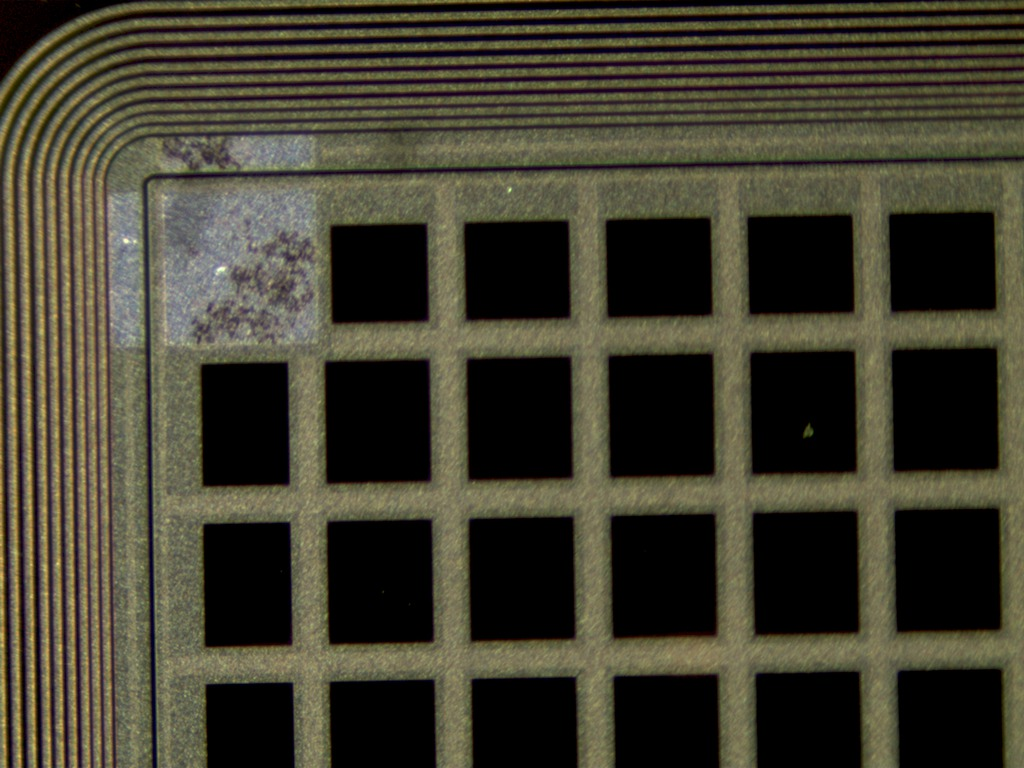
\includegraphics[width=0.4\textwidth]{ch7/vis_insp_2}
  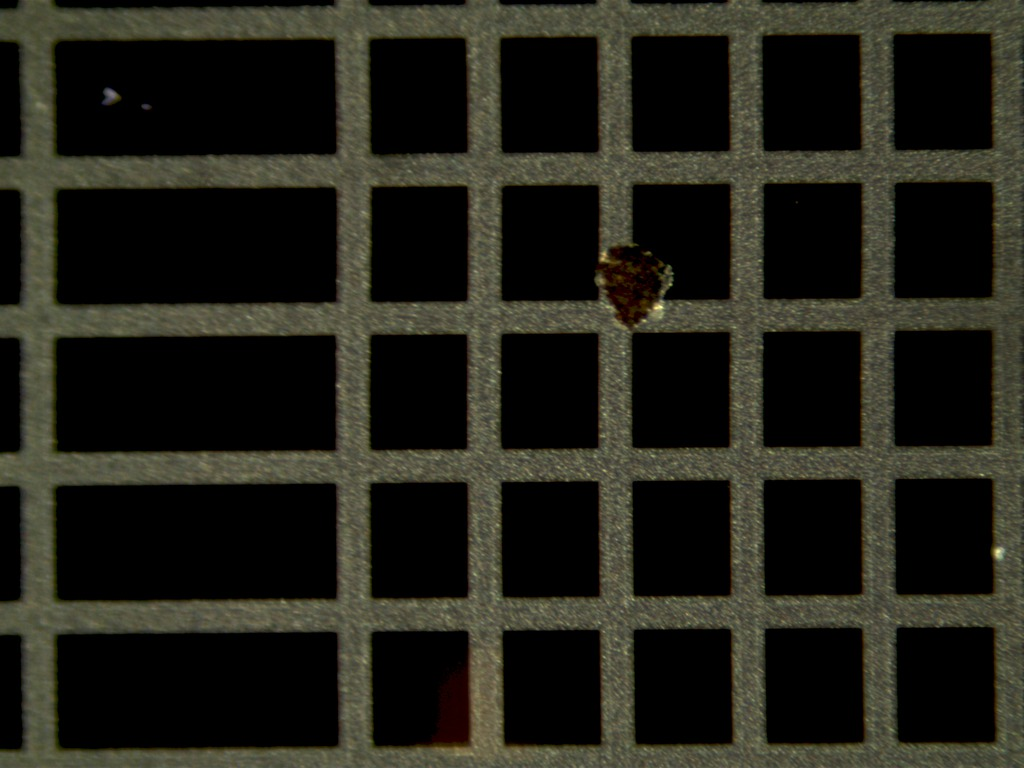
\includegraphics[width=0.4\textwidth]{ch7/vis_insp_3}
  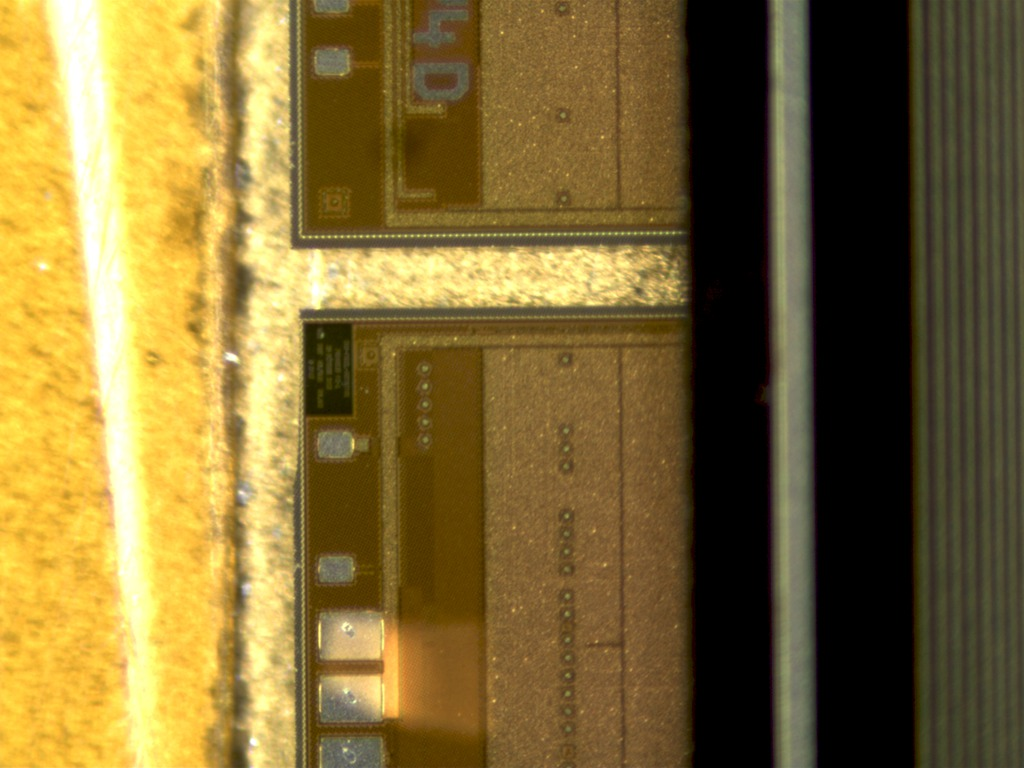
\includegraphics[width=0.4\textwidth]{ch7/vis_insp_5}
  \caption[Visual inspection of a bare module.]{Photograph of the visual inspection of a BBM showing few of the things observed during a visual inspection: A good module (top left), scratches on the high voltage connection path (top right), scratch on the midle of the BBM (bottom left), and scratches on the wire bonds pad (bottom right)}\label{fig:vis_insp_bbm}
\end{figure}

\begin{figure}[!h]
  \centering
  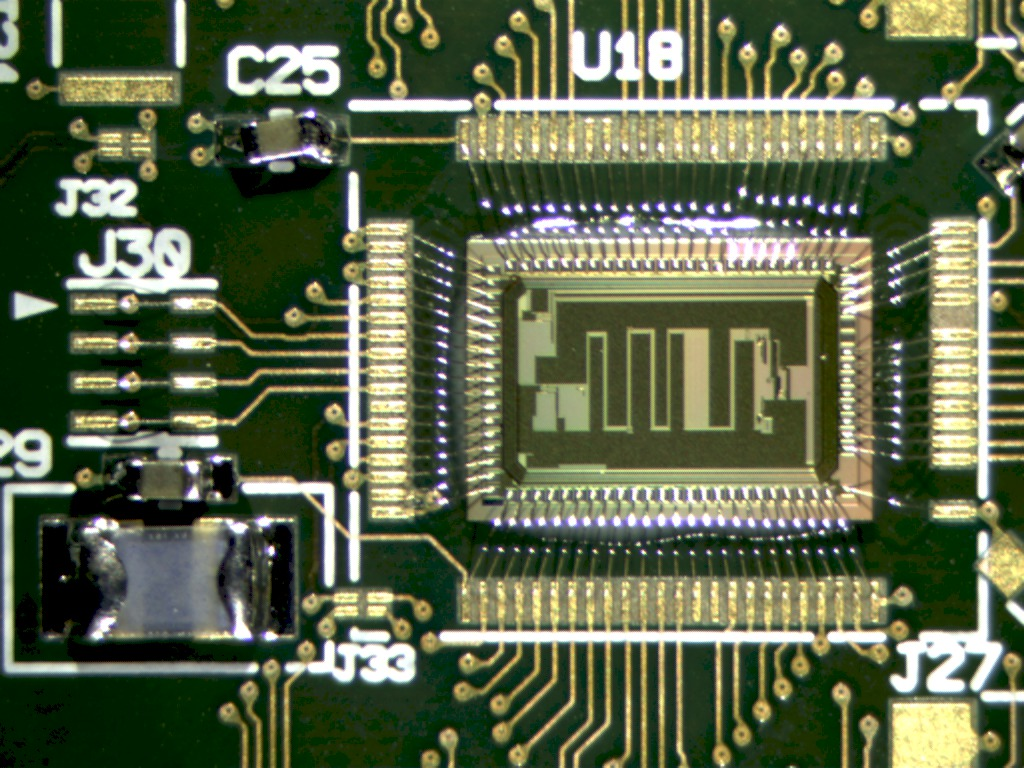
\includegraphics[width=0.4\textwidth]{ch7/hdi_tbm}
  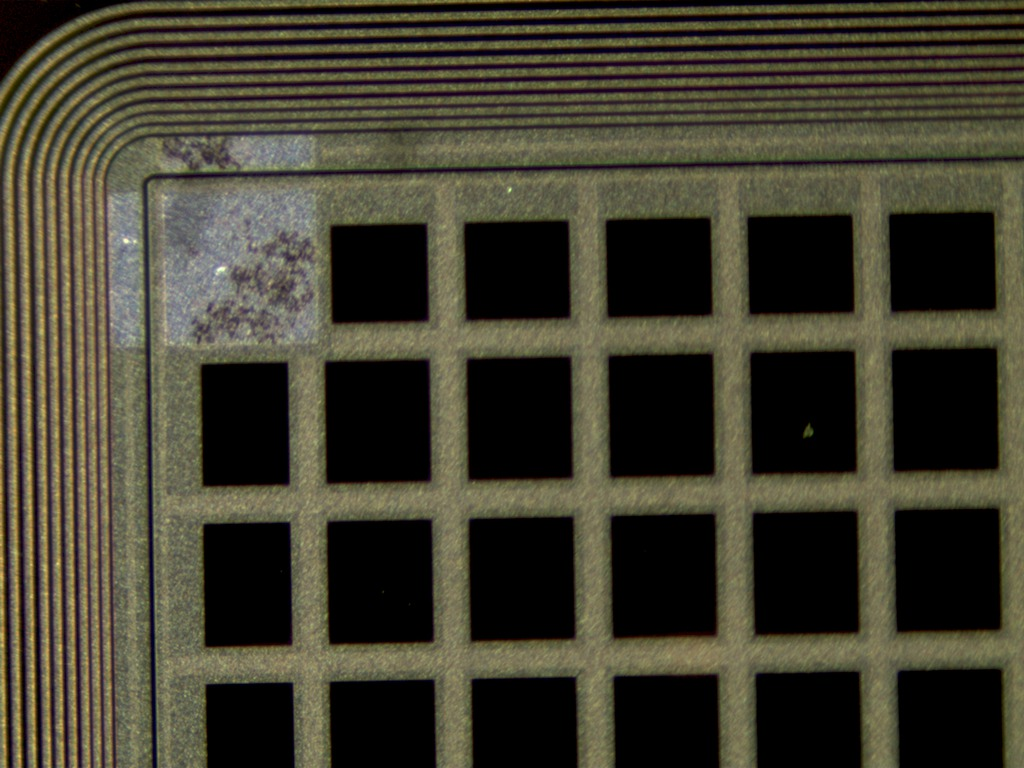
\includegraphics[width=0.4\textwidth]{ch7/vis_insp_2}
  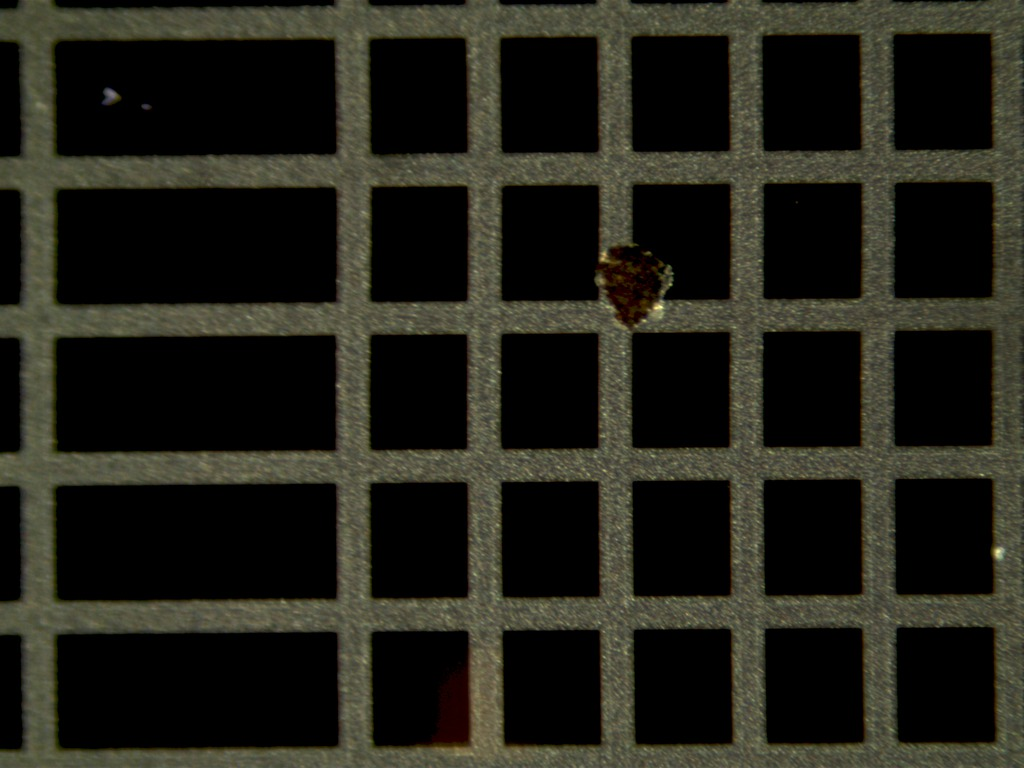
\includegraphics[width=0.4\textwidth]{ch7/vis_insp_3}
  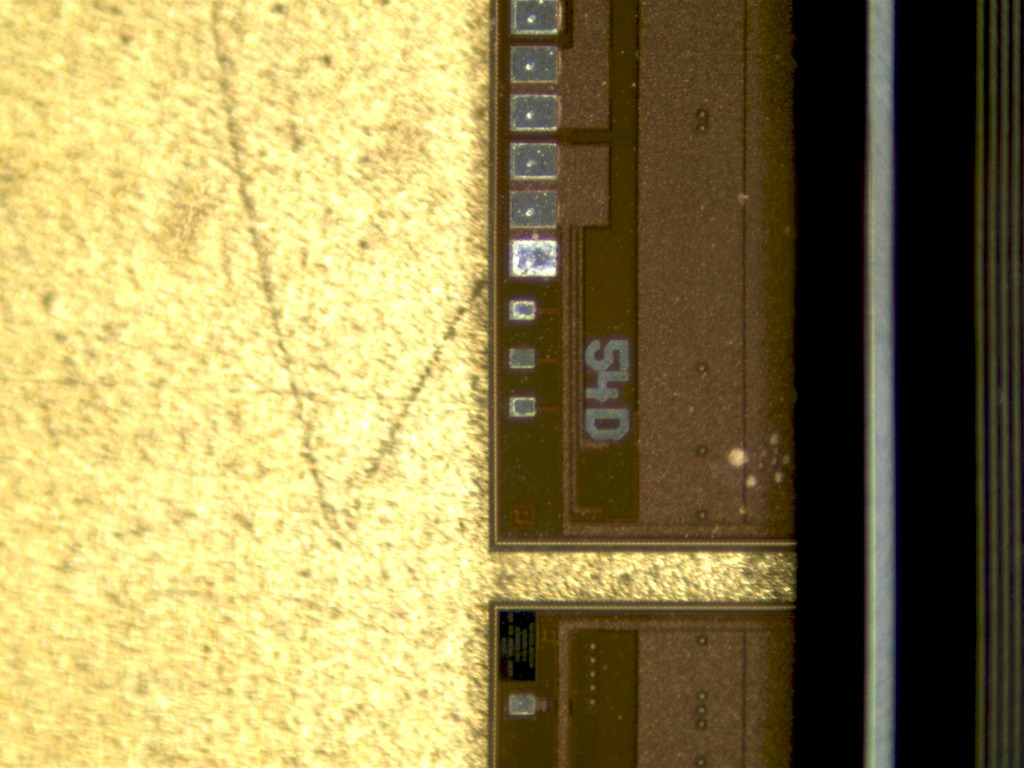
\includegraphics[width=0.4\textwidth]{ch7/vis_insp_4}
  \caption[Visual inspection of a bare module.]{Photograph of the visual inspection of a BBM showing few of the things observed during a visual inspection: A good module (top left), scratches on the high voltage connection path (top right), scratch on the midle of the BBM (bottom left), and scratches on the wire bonds pad (bottom right)}\label{fig:vis_insp_hdi}
\end{figure}

In general more unusual features were found on BBMs than on HDI. 





{\rojo{why BBM has more scratches than the HDI?}}

\subsection{IV Test}
After both BBM and HDI were visually inspected 

\begin{figure}[!h]
  \centering
  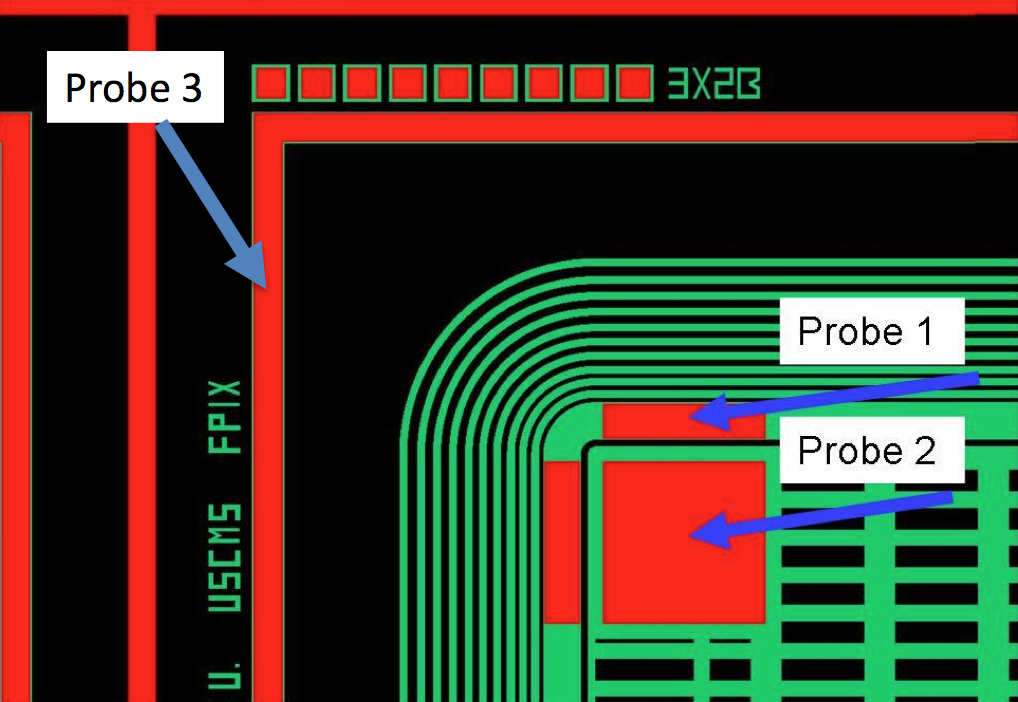
\includegraphics[width=0.7\textwidth]{ch7/sensor_probe_positions}
  \caption[Probe position for an IV test]{Probe position for an IV test on a BBM.}\label{fig:sensor_probe_positions}
\end{figure}

\begin{figure}[!h]
  \centering
  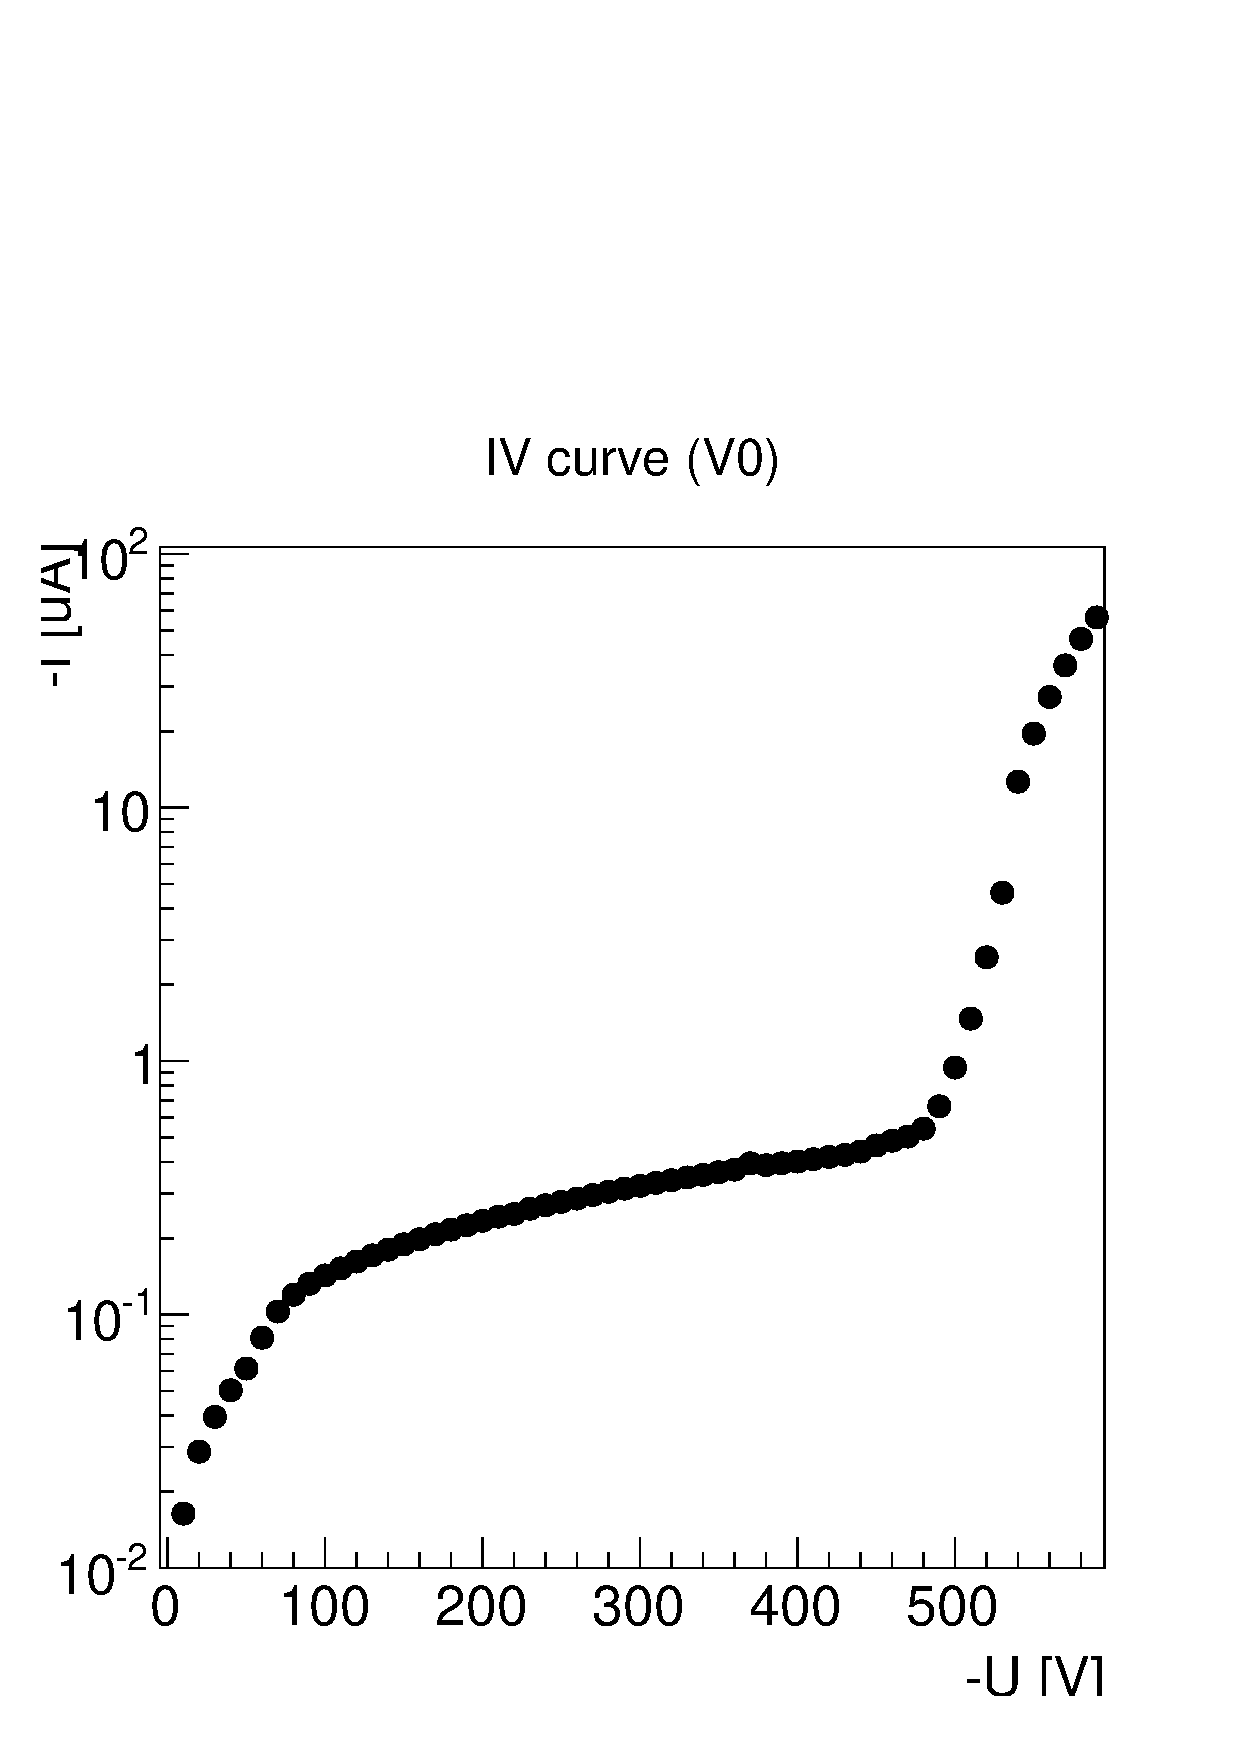
\includegraphics[width=0.4\textwidth]{ch7/iv_test}
  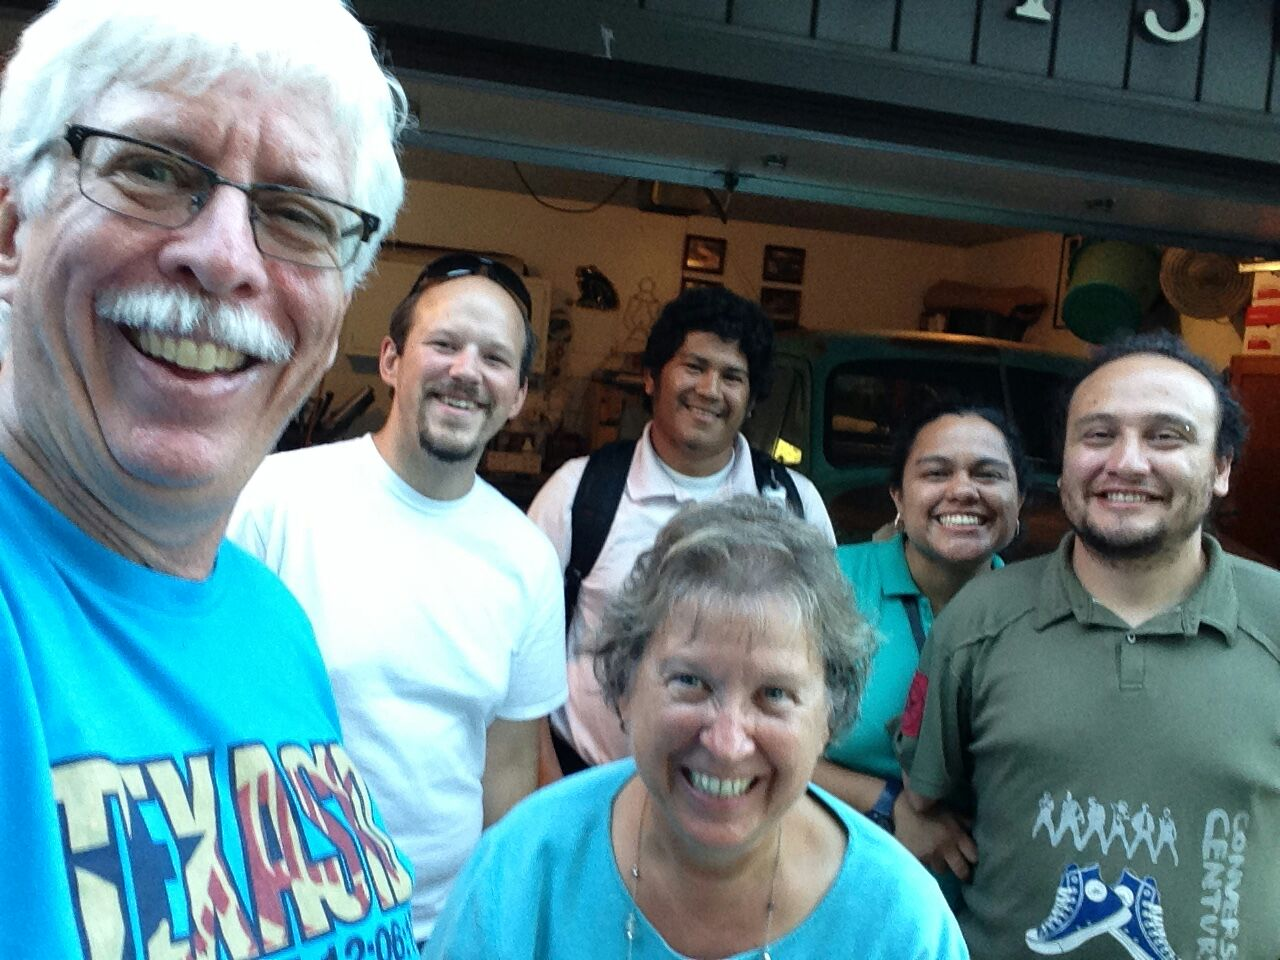
\includegraphics[width=0.4\textwidth]{ch7/12}
  \caption[IV result of a BBM]{IV good and bad.}\label{fig:vis_insp}
\end{figure}

\subsection{Gluing}
The International Flat Earth Research Society (IFERS), better known as the Flat Earth Society, was set up by Samuel Shenton in 1956, in Dover, UK, as a direct descendant of the Universal Zetetic Society. This was just before the Soviet Union launched the first artificial satellite, Sputnik; he responded: "Would sailing round the Isle of Wight prove that it were spherical? It is just the same for those satellites."

His primary aim was to reach children before they were convinced about a spherical Earth. Despite plenty of publicity, the space race eroded Shenton's support in Britain until 1967, when he started to become famous due to the Apollo program.
\begin{figure}[!h]
  \centering
  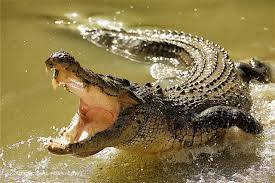
\includegraphics[width=0.7\textwidth]{ch7/11}
  \caption[Gluing routine]{Gluing routine}\label{fig:vis_insp}
\end{figure}


\subsection{Wirebonding}
Homer Wells es un huérfano al que no le falta familia. Ha crecido en el orfanato de St. Cloud's bajo la poco convencional pero tierna tutela del Dr. Wilbur que nunca ha dejado de dar afecto a sus chicos. Pero a medida que Homer se va haciendo un hombre y se da cuenta del gran abanico de posibilidades que le  pero tierna tutela del Dr. Wilbur que nunca ha dejado de dar afecto a sus chicos. Pero a medida que Homer se va haciendo un hombre y se da cuenta del gran abanico de posibilidades que le brinda la vida, empieza a dudar y a cuestionar los métodos del Dr. Wilbur.

\begin{figure}[!h]
  \centering
  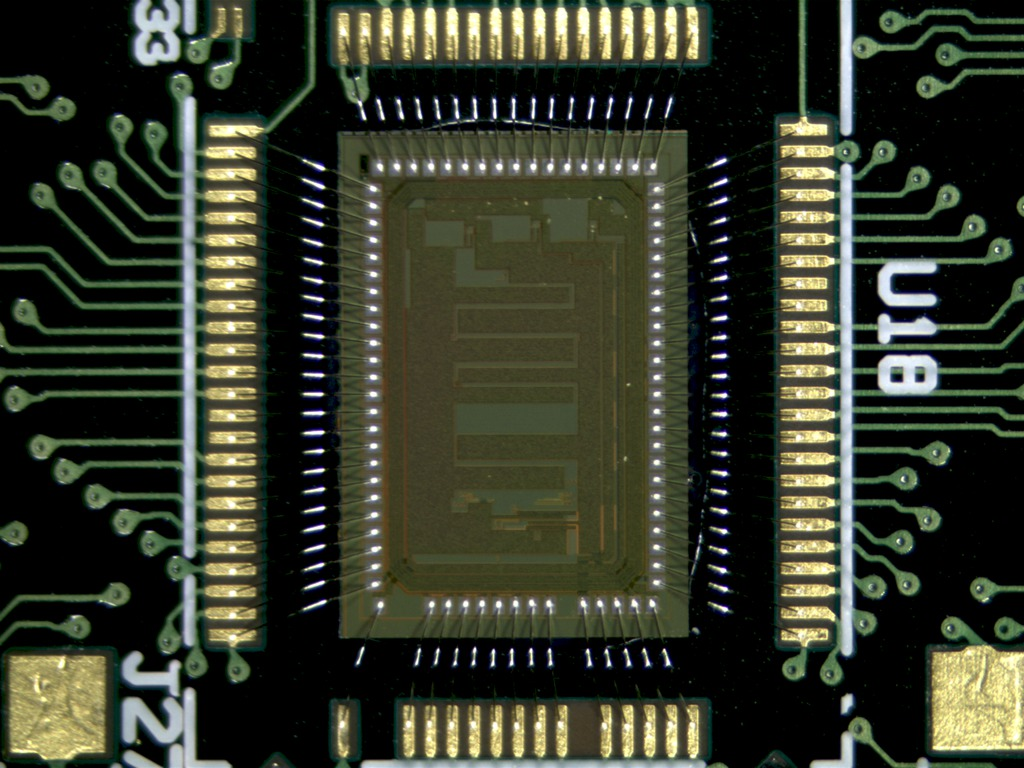
\includegraphics[width=0.7\textwidth]{ch7/9}
  \caption[bla for index.]{bla bla.}\label{fig:vis_insp}
\end{figure}

brinda la vida, empieza a dudar y a cuestionar los métodos del Dr. Wilbur. Homer Wells es un huérfano al que no le falta familia. Ha crecido en el orfanato de St. Cloud's bajo la poco convencional

\begin{figure}[!h]
  \centering
  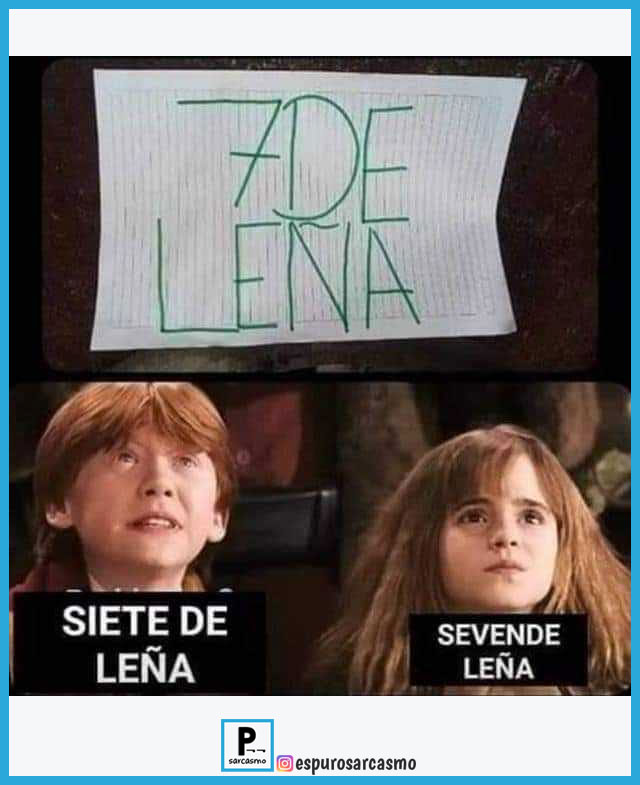
\includegraphics[width=0.7\textwidth]{ch7/13}
  \caption[bla for index.]{bla bla.}\label{fig:vis_insp}
\end{figure}

\subsection{Encapsulation}
The International Flat Earth Research Society (IFERS), better known as the Flat Earth Society, was set up by Samuel Shenton in 1956, in Dover, UK, as a direct descendant of the Universal Zetetic Society. This was just before the Soviet Union launched the first artificial satellite, Sputnik; he responded: "Would sailing round the Isle of Wight prove that it were spherical? It is just the same for those satellites."

\begin{figure}[!h]
  \centering
  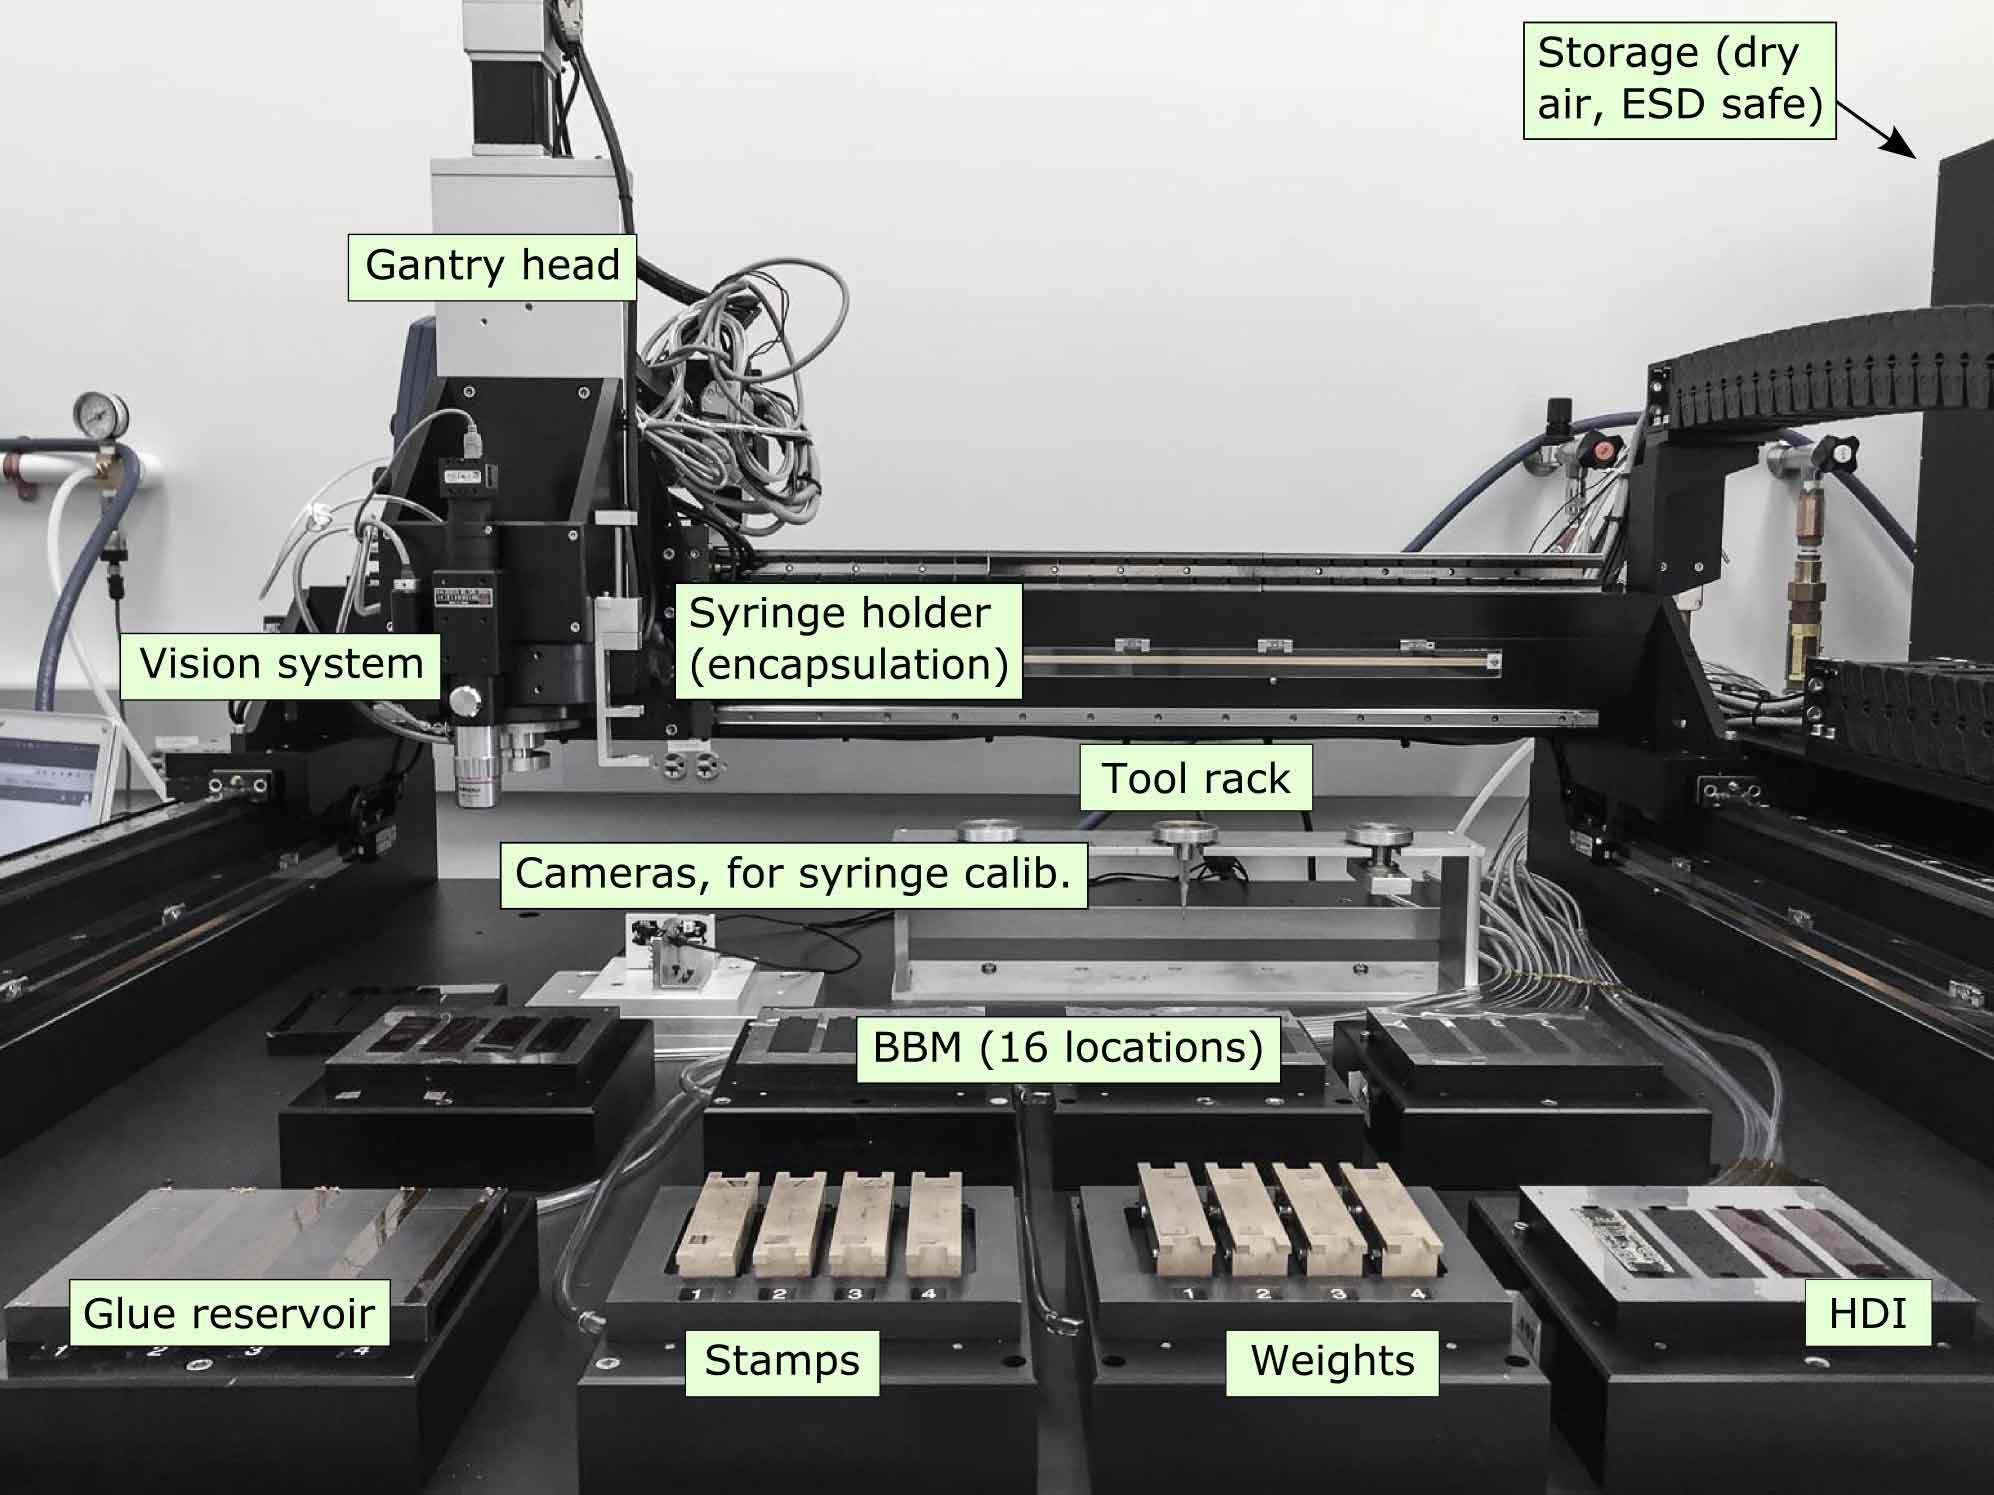
\includegraphics[width=0.7\textwidth]{../images/ch7/gantry}
  \caption[bla for index.]{bla bla.}\label{fig:gantry}
\end{figure}



\subsection{Electrical Test of a Fully assembly Module}
The International Flat Earth Research Society (IFERS), better known as the Flat Earth Society, was set up by Samuel Shenton in 1956, in Dover, UK, as a direct descendant of the Universal Zetetic Society. This was just before the Soviet Union launched the first artificial satellite, Sputnik; he responded: "Would sailing round the Isle of Wight prove that it were spherical? It is just the same for those satellites."

His primary aim was to reach children before they were convinced about a spherical Earth. Despite plenty of publicity, the space race eroded Shenton's support in Britain until 1967, when he started to become famous due to the Apollo program.
\begin{figure}[!h]
  \centering
  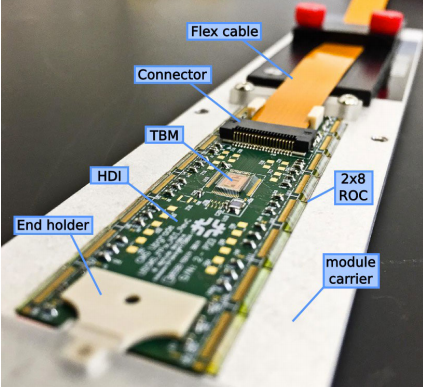
\includegraphics[width=0.7\textwidth]{../images/ch7/fully_asem_mod}
  \caption[Fully assembly Module]{Fully assembly Module}\label{fig:fully_asem_mod}
\end{figure}

\subsubsection{Pretest}
The International Flat Earth Research Society (IFERS), better known as the Flat Earth Society, was set up by Samuel Shenton in 1956, in Dover, UK, as a direct descendant of the Universal Zetetic Society. This was just before the Soviet Union launched the first artificial satellite, Sputnik; he responded: "Would sailing round the Isle of Wight prove that it were spherical? It is just the same for those satellites."

His primary aim was to reach children before they were convinced about a spherical Earth. Despite plenty of publicity, the space race eroded Shenton's support in Britain until 1967, when he started to become famous due to the Apollo program.
\begin{figure}[!h]
  \centering
  
\includegraphics[width=0.7\textwidth]{../images/ch7/1}
  \caption[Visual inspection of a bare module.]{Visual inspection of a bare module.}\label{fig:vis_insp}
\end{figure}

\begin{figure}[!h]
  \centering
  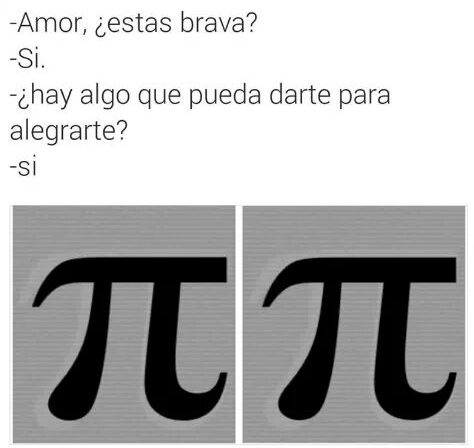
\includegraphics[width=0.7\textwidth]{../images/ch7/8}
  \caption[Electrical test station]{Electrical test station.}\label{fig:vis_insp}
\end{figure}

\subsubsection{Pretest}
The International Flat Earth Research Society (IFERS), better known as the Flat Earth Society, was set up by Samuel Shenton in 1956, in Dover, UK, as a direct descendant of the Universal Zetetic Society. This was just before the Soviet Union launched the first artificial satellite, Sputnik; he responded: "Would sailing round the Isle of Wight prove that it were spherical? It is just the same for those satellites."

His primary aim was to reach children before they were convinced about a spherical Earth. Despite plenty of publicity, the space race eroded Shenton's support in Britain until 1967, when he started to become famous due to the Apollo program.
\begin{figure}[!h]
  \centering
  
\includegraphics[width=0.7\textwidth]{../images/ch7/2}
  \caption[Pretest]{Pretest.}\label{fig:vis_insp}
\end{figure}

\subsubsection{Pixel Alive}
The International Flat Earth Research Society (IFERS), better known as the Flat Earth Society, was set up by Samuel Shenton in 1956, in Dover, UK, as a direct descendant of the Universal Zetetic Society. This was just before the Soviet Union launched the first artificial satellite, Sputnik; he responded: "Would sailing round the Isle of Wight prove that it were spherical? It is just the same for those satellites."

His primary aim was to reach children before they were convinced about a spherical Earth. Despite plenty of publicity, the space race eroded Shenton's support in Britain until 1967, when he started to become famous due to the Apollo program.
\begin{figure}[!h]
  \centering
  
\includegraphics[width=0.7\textwidth]{../images/ch7/3}
  \caption[Pixel alive.]{Pixel alive good and bad.}\label{fig:vis_insp}
\end{figure}

\subsubsection{Trim Test}
The International Flat Earth Research Society (IFERS), better known as the Flat Earth Society, was set up by Samuel Shenton in 1956, in Dover, UK, as a direct descendant of the Universal Zetetic Society. This was just before the Soviet Union launched the first artificial satellite, Sputnik; he responded: "Would sailing round the Isle of Wight prove that it were spherical? It is just the same for those satellites."

His primary aim was to reach children before they were convinced about a spherical Earth. Despite plenty of publicity, the space race eroded Shenton's support in Britain until 1967, when he started to become famous due to the Apollo program.
\begin{figure}[!h]
  \centering
  
\includegraphics[width=0.7\textwidth]{../images/ch7/4}
  \caption[Trim test.]{Trim test of a faulty and working module.}\label{fig:vis_insp}
\end{figure}

\subsubsection{PH Optimization}
The International Flat Earth Research Society (IFERS), better known as the Flat Earth Society, was set up by Samuel Shenton in 1956, in Dover, UK, as a direct descendant of the Universal Zetetic Society. This was just before the Soviet Union launched the first artificial satellite, Sputnik; he responded: "Would sailing round the Isle of Wight prove that it were spherical? It is just the same for those satellites."

His primary aim was to reach children before they were convinced about a spherical Earth. Despite plenty of publicity, the space race eroded Shenton's support in Britain until 1967, when he started to become famous due to the Apollo program.
\begin{figure}[!h]
  \centering
  
\includegraphics[width=0.7\textwidth]{../images/ch7/5}
  \caption[Ph Optimization.]{PH optimization.}\label{fig:vis_insp}
\end{figure}

\subsubsection{Gain Pedestal}
The International Flat Earth Research Society (IFERS), better known as the Flat Earth Society, was set up by Samuel Shenton in 1956, in Dover, UK, as a direct descendant of the Universal Zetetic Society. This was just before the Soviet Union launched the first artificial satellite, Sputnik; he responded: "Would sailing round the Isle of Wight prove that it were spherical? It is just the same for those satellites."

His primary aim was to reach children before they were convinced about a spherical Earth. Despite plenty of publicity, the space race eroded Shenton's support in Britain until 1967, when he started to become famous due to the Apollo program.
\begin{figure}[!h]
  \centering
  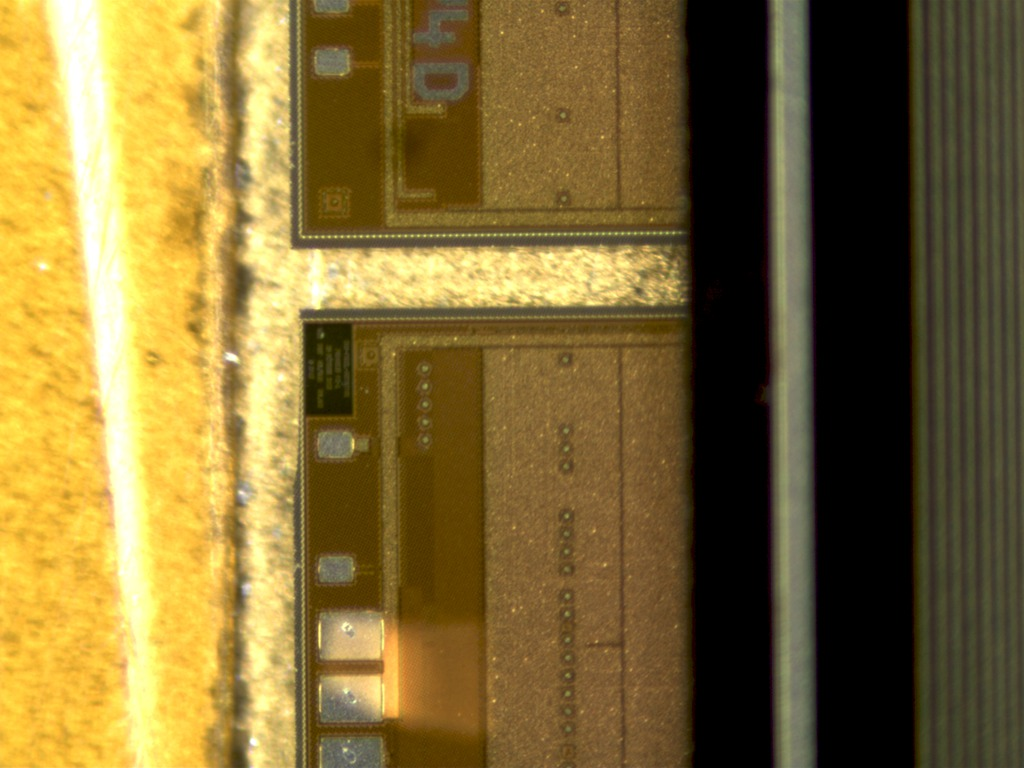
\includegraphics[width=0.7\textwidth]{../images/ch7/6}
  \caption[Gain Pedestal.]{Gain pedestal.}\label{fig:vis_insp}
\end{figure}

\subsubsection{Bond Bonding Test}
The International Flat Earth Research Society (IFERS), better known as the Flat Earth Society, was set up by Samuel Shenton in 1956, in Dover, UK, as a direct descendant of the Universal Zetetic Society. This was just before the Soviet Union launched the first artificial satellite, Sputnik; he responded: "Would sailing round the Isle of Wight prove that it were spherical? It is just the same for those satellites."

His primary aim was to reach children before they were convinced about a spherical Earth. Despite plenty of publicity, the space race eroded Shenton's support in Britain until 1967, when he started to become famous due to the Apollo program.
\begin{figure}[!h]
  \centering
  
\includegraphics[width=0.7\textwidth]{../images/ch7/7}
  \caption[Bond bonding test.]{Bond bonding test.}\label{fig:vis_insp}
\end{figure}

\begin{figure}[!h]
  \centering
  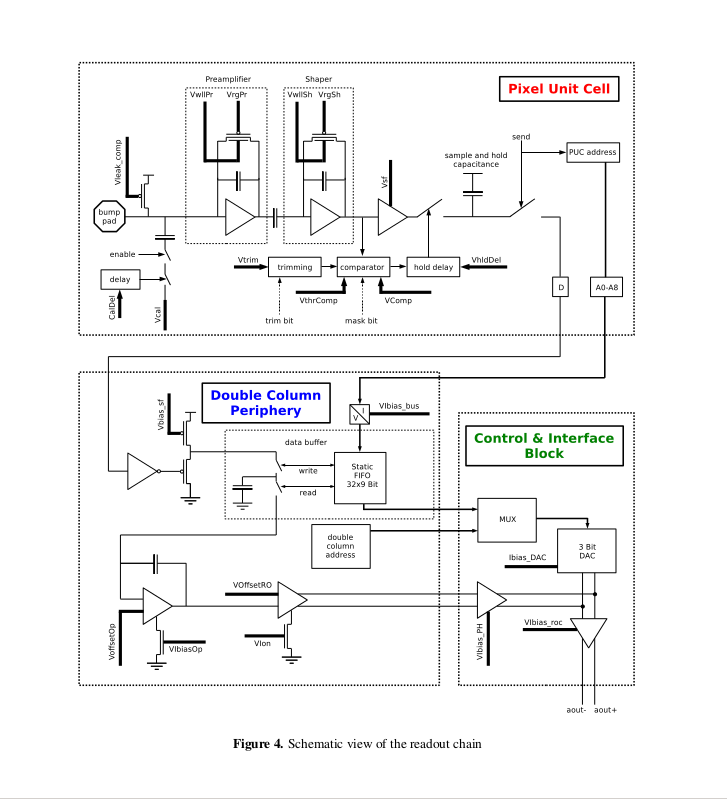
\includegraphics[width=0.7\textwidth]{../images/ch7/pix_unit_cell}
  \caption[bla for index.]{bla bla.}\label{fig:pix_unit_cell}
\end{figure}



\begin{figure}[!h]
  \centering
  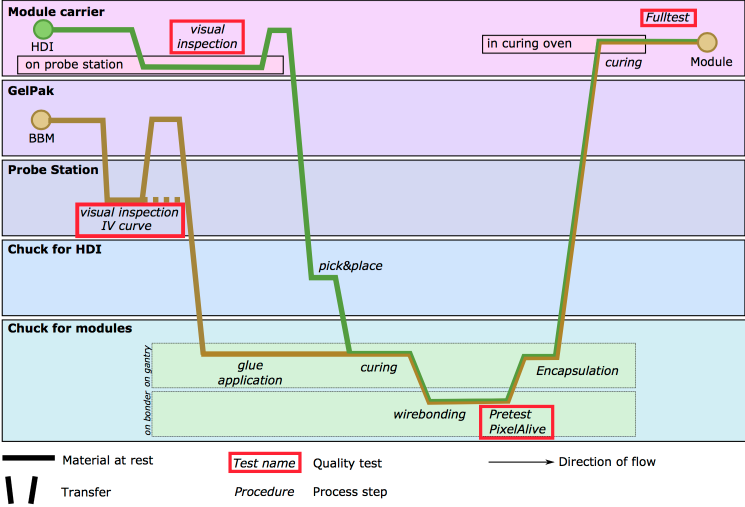
\includegraphics[width=0.7\textwidth]{../images/ch7/unl_workflow2}
  \caption[bla for index.]{bla bla.}\label{fig:unl_workflow2}
\end{figure}
